\newpage
\subsection{Caso d'uso UC8: Gestione delle domande}
	\label{UC8}
	\begin{figure}[ht]
		\centering
			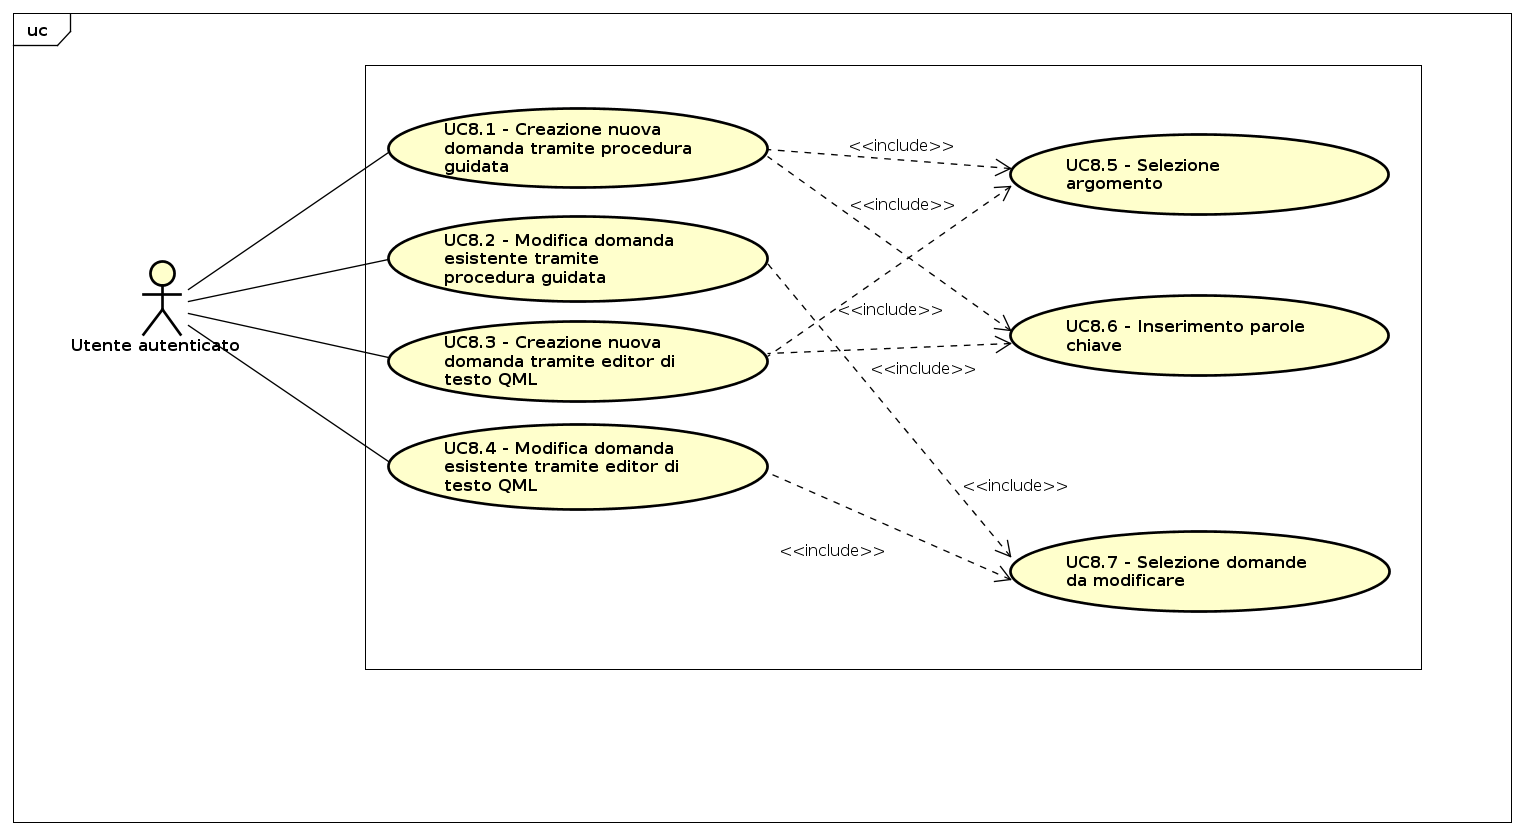
\includegraphics[scale=0.45,keepaspectratio]{UML/UC8.png}
		\caption{UC8: Gestione delle domande}
	\end{figure}
	\FloatBarrier
	\begin{itemize}
		\item
			\textbf{Attori}: utente autenticato, utente autenticato pro;
		\item		
			\textbf{Descrizione}: l'attore può creare e modificare domande;
		\item
			\textbf{Precondizione}: il sistema ha riconosciuto l'autenticazione dell'attore; 
		\item
			\textbf{Postcondizione}: l'attore ha compiuto una delle operazioni appartenenti a questa funzionalità;
		\item
			\textbf{Scenario principale}:
	       		\begin{enumerate}
					\item
					L'attore crea una nuova domanda tramite procedura guidata (UC8.1);
					\item
					L'attore modifica una domanda tramite procedura guidata (UC8.2);
					\item
					L'attore crea una nuova domanda tramite editor di testo \textit{QML\ped{G}} (UC8.3);
					\item
					L'attore modifica una domanda tramite editor di testo \textit{QML\ped{G}} (UC8.4).
	 			\end{enumerate}
		\item \textbf{Inclusioni}: 
			\begin{enumerate}
				\item L'attore può selezionare un argomento da assegnare alla domanda (UC8.5);
				\item L'attore può selezionare delle parole chiave da assegnare alle domande (UC8.6);								\item L'attore può selezionare la domanda da modificare (UC8.7);
			\end{enumerate}
	\end{itemize}
	\subsubsection{Caso d'uso UC8.1: Creazione nuova domanda tramite procedura guidata}
	\label{UC8.1}
	\begin{figure}[h]
		\centering
			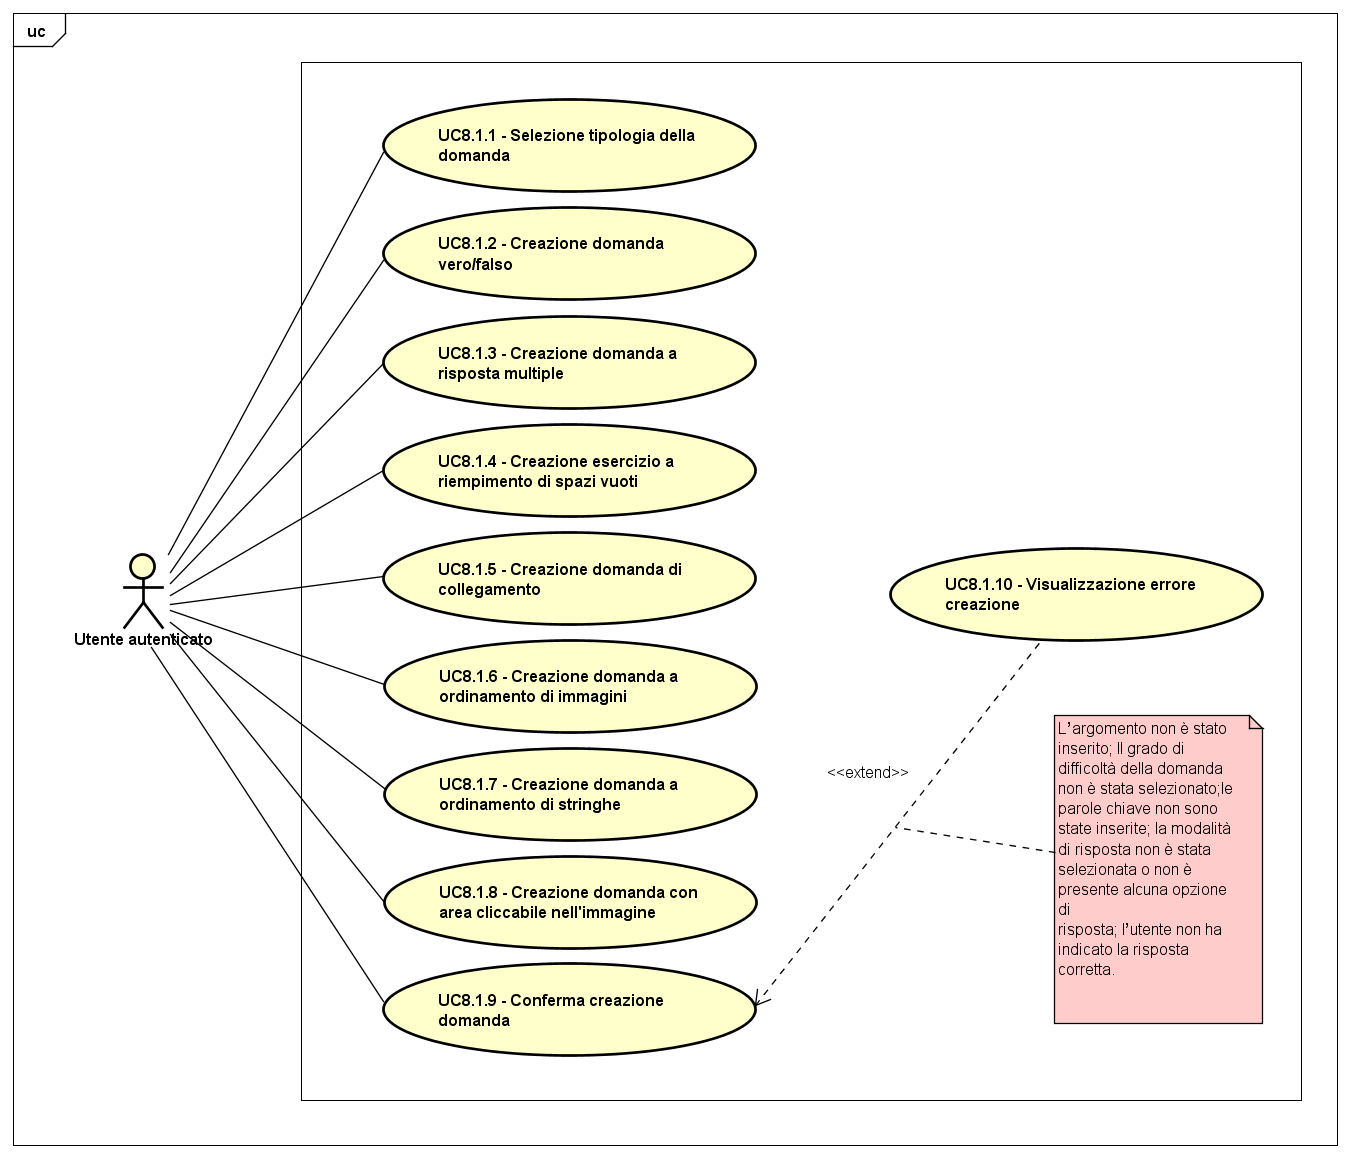
\includegraphics[scale=0.45,keepaspectratio]{UML/UC8_1.png}
		\caption{UC8.1: Creazione nuova domanda tramite procedura guidata}
	\end{figure}
	\FloatBarrier
	\begin{itemize}
		\item
			\textbf{Attori}: utente autenticato, utente autenticato pro;
		\item		
			\textbf{Descrizione}: l'attore può creare una nuova domanda tramite procedura guidata;
		\item
			\textbf{Precondizione}: il sistema presenta la funzionalità di creazione della domanda;
		\item
			\textbf{Postcondizione}: l'attore crea una domanda;		
		\item
			\textbf{Scenario principale}:
	       		\begin{enumerate}
					\item
					L'attore può selezionare la tipologia di domanda (UC8.1.1);
					\item
					L'attore può richiamare il \textit{wizard\ped{G}} per creare una domanda vero/falso (UC8.1.2);
					\item
					L'attore può richiamare il \textit{wizard\ped{G}} per creare una domanda a risposta multipla \\(UC8.1.3);
					\item
					L'attore può richiamare il \textit{wizard\ped{G}} per creare un esercizio a riempimento di spazi vuoti (UC8.1.4);
					\item
					L'attore può richiamare il \textit{wizard\ped{G}} per creare una domanda di collegamento (UC8.1.5);
					\item
					L'attore può richiamare il \textit{wizard\ped{G}} per creare una domanda a ordinamento di immagini (UC8.1.6);
					\item
					L'attore può richiamare il \textit{wizard\ped{G}} per creare una domanda a ordinamento di stringhe (UC8.1.7);
					\item
					L'attore può richiamare il \textit{wizard\ped{G}} per creare una domanda con area cliccabile nell'immagine (UC8.1.8);
					\item
					L'attore può confermare la creazione della domanda (UC8.1.9).
	 			\end{enumerate}
	 	\item
			\textbf{Estensioni}: l'attore visualizza un messaggio d'errore relativo alla creazione della domanda (UC8.1.10).
	\end{itemize}

	\subsubsection{Caso d'uso UC8.1.1: Selezione tipologia di domanda}
	\begin{itemize}
		\item
			\textbf{Attori}: utente autenticato, utente autenticato pro;
		\item
			\textbf{Descrizione}: l'attore può scegliere la tipologia di domanda che vuole inserire;
		\item		
			\textbf{Precondizione}: il sistema presenta la funzionalità di selezionare una tipologia di una domanda;
		\item
			\textbf{Postcondizione}: l'utente ha selezionato la tipologia di domanda da inserire;
		\item 
			\textbf{Scenario principale}: l'utente seleziona la tipologia di domanda.
	\end{itemize}

	%inclusione file latex wizard
\subsubsection{Caso d'uso UC8.1.2: Creazione domanda vero/falso}
	\label{UC8.1.2}
	\begin{figure}[h]
		\centering
			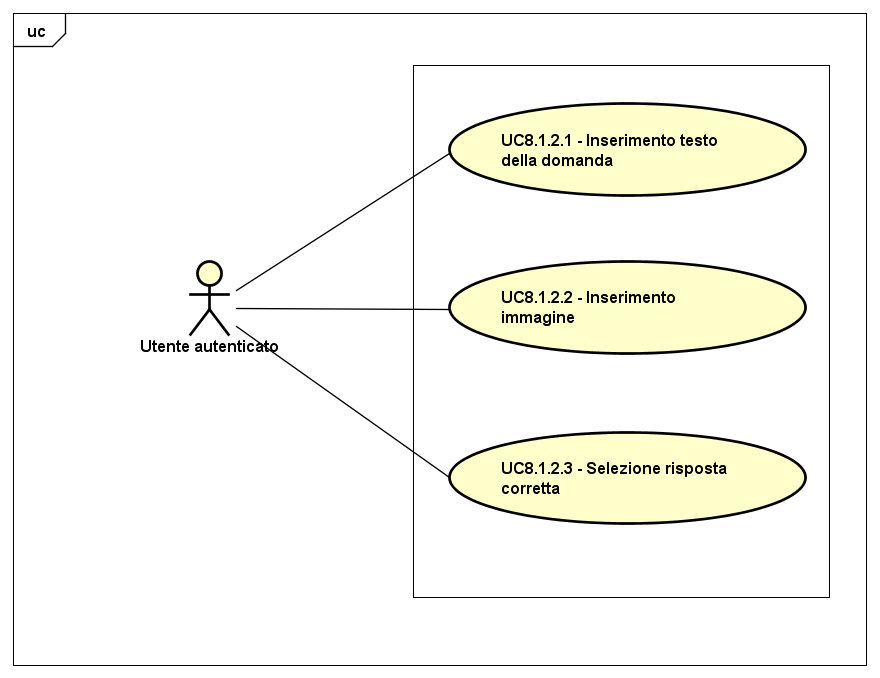
\includegraphics[scale=0.45,keepaspectratio]{UML/UC8_1_2.png}
		\caption{UC8.1.2: Creazione domanda vero/falso}
	\end{figure}
	\FloatBarrier
	\begin{itemize}
		\item
			\textbf{Attori}: utente autenticato, utente autenticato pro;
		\item		
			\textbf{Descrizione}: l'attore può utilizzare la procedura guidata per la creazione di una domanda vero/falso;
		\item
			\textbf{Precondizione}: il sistema presenta all'attore la procedura guidata per la creazione di una domanda vero/falso; 
		\item
			\textbf{Postcondizione}: l'attore ha creato una domanda vero/falso;
		\item
			\textbf{Scenario principale}:
	       		\begin{enumerate}
	       			\item
	       			L'attore può inserire il testo della domanda (UC8.1.2.1);
	       			\item
	       			L'attore può inserire un'immagine relativa al testo della domanda (UC8.1.2.2);
					\item
					L'attore può indicare la risposta corretta tramite uno strumento di selezione (UC8.1.2.3).
	 			\end{enumerate}
	\end{itemize}

\subsubsection{Caso d'uso UC8.1.2.1: Inserimento testo della domanda}
	\begin{itemize}
		\item
			\textbf{Attori}: utente autenticato, utente autenticato pro;
		\item		
			\textbf{Descrizione}: l'attore può inserire il testo della domanda;
		\item
			\textbf{Precondizione}: il sistema presenta all'attore lo spazio destinato all'inserimento del testo della domanda; 
		\item
			\textbf{Postcondizione}: l'attore ha inserito il testo della domanda;
		\item
			\textbf{Scenario principale}: l'attore inserisce il testo della domanda. 
	 			
	\end{itemize}
	
\subsubsection{Caso d'uso UC8.1.2.2: Inserimento immagine}
	\begin{itemize}
		\item
			\textbf{Attori}: utente autenticato, utente autenticato pro;
		\item		
			\textbf{Descrizione}: l'attore può inserire un'immagine relativa al testo della domanda;
		\item
			\textbf{Precondizione}: il sistema presenta all'attore la funzionalità di inserimento di un immagine; 
		\item
			\textbf{Postcondizione}: l'attore ha inserito un'immagine relativa al testo della domanda;
		\item
			\textbf{Scenario principale}: l'attore inserisce un'immagine.						
	\end{itemize}
	

\subsubsection{Caso d'uso UC8.1.2.3: Selezione risposta corretta}
	\begin{itemize}
		\item
			\textbf{Attori}: utente autenticato, utente autenticato pro;
		\item		
			\textbf{Descrizione}: l'attore può indicare la risposta corretta;
		\item
			\textbf{Precondizione}: il sistema presenta all'attore la funzionalità di selezione di una risposta corretta; 
		\item
			\textbf{Postcondizione}: l'attore ha selezionato la risposta corretta;
		\item
			\textbf{Scenario principale}: l'attore indica la risposta corretta.  			
	\end{itemize}
\subsubsection{Caso d'uso UC8.1.3: Creazione domanda a risposta multipla}
	\label{UC8.1.3}
	\begin{figure}[ht]
		\centering
			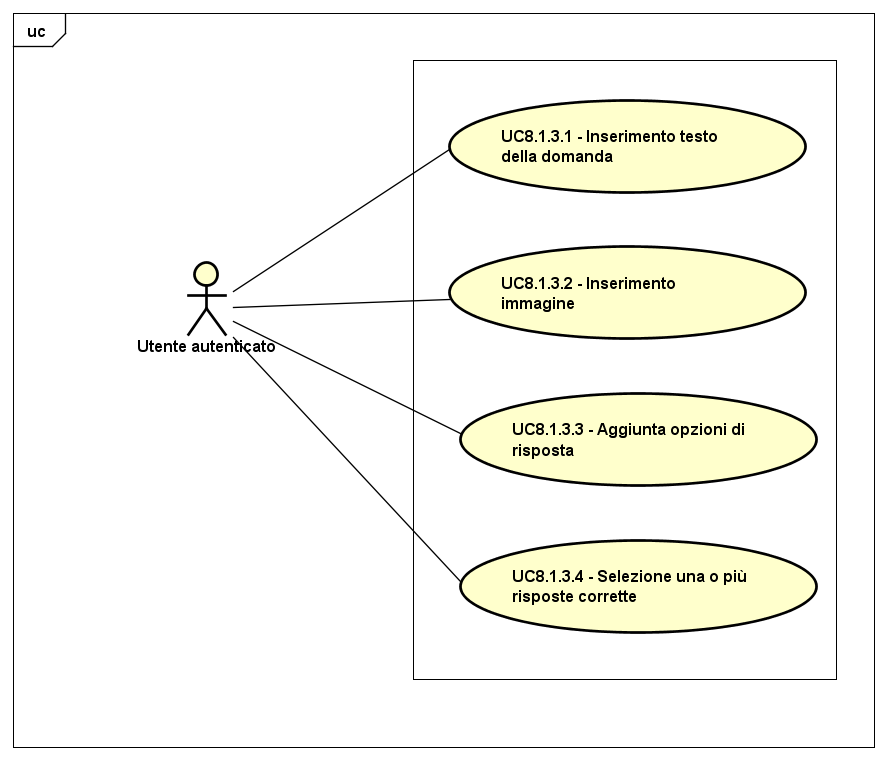
\includegraphics[scale=0.45,keepaspectratio]{UML/UC8_1_3.png}
		\caption{UC8.1.3: Creazione domanda a risposta multipla}
	\end{figure}
	\FloatBarrier
	\begin{itemize}
		\item
			\textbf{Attori}: utente autenticato, utente autenticato pro;
		\item		
			\textbf{Descrizione}: l'attore può utilizzare la procedura guidata per la creazione di una domanda a risposta multipla;
		\item
			\textbf{Precondizione}: il sistema presenta all'attore la procedura guidata per la creazione di una domanda a risposta multipla;
		\item
			\textbf{Postcondizione}: l'attore ha creato una domanda a risposta multipla;
		\item
			\textbf{Scenario principale}:
	       		\begin{enumerate}
	       			\item
	       			L'attore può inserire il testo della domanda (UC8.1.3.1);
	       			\item
	       			L'attore può inserire un'immagine relativa al testo della domanda (UC8.1.3.2);
	       			\item
	       			L'attore può aggiungere almeno due opzioni di risposta (UC8.1.3.3);
					\item
					L'attore può indicare una o più risposte corrette (UC8.1.3.4).
	 			\end{enumerate}
	\end{itemize}

\subsubsection{Caso d'uso UC8.1.3.1: Inserimento testo della domanda}
	\begin{itemize}
		\item
			\textbf{Attori}: utente autenticato, utente autenticato pro;
		\item		
			\textbf{Descrizione}: l'attore può inserire il testo della domanda;
		\item
			\textbf{Precondizione}: il sistema presenta all'attore lo spazio destinato all'inserimento del testo della domanda;
		\item
			\textbf{Postcondizione}: l'attore ha inserito il testo della domanda;
		\item
			\textbf{Scenario principale}: l'attore inserisce il testo della domanda. 
	 			
	\end{itemize}
	
\subsubsection{Caso d'uso UC8.1.3.2: Inserimento immagine}
	\begin{itemize}
		\item
			\textbf{Attori}: utente autenticato, utente autenticato pro;
		\item		
			\textbf{Descrizione}: l'attore può inserire un'immagine relativa al testo della domanda;
		\item
			\textbf{Precondizione}: il sistema presenta all'attore la funzionalità di inserimento di un immagine; 
		\item
			\textbf{Postcondizione}: l'attore ha inserito un'immagine relativa al testo della domanda;
		\item
			\textbf{Scenario principale}: l'attore inserisce l'immagine.						
	\end{itemize}


	
\subsubsection{Caso d'uso UC8.1.3.3: Aggiunta opzioni di risposta}
	\label{UC8.1.3.3}
	\begin{figure}[h]
		\centering
			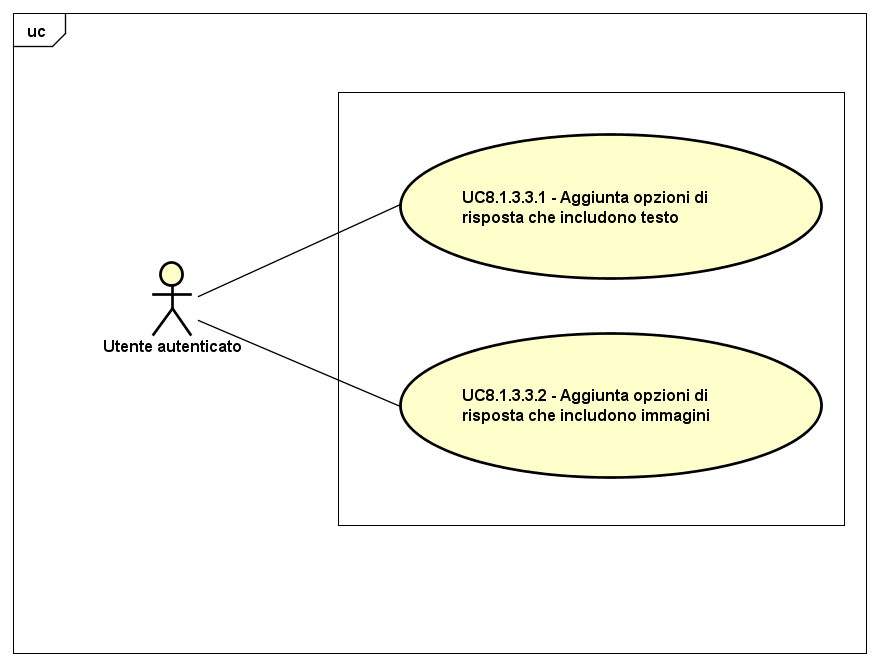
\includegraphics[scale=0.45,keepaspectratio]{UML/UC8_1_3_3.png}
		\caption{UC8.1.3.3: Aggiunta opzioni di risposta}
	\end{figure}
	\FloatBarrier
	\begin{itemize}
		\item
			\textbf{Attori}: utente autenticato, utente autenticato pro;
		\item		
			\textbf{Descrizione}: l'attore può aggiungere almeno due opzioni di risposta;
		\item
			\textbf{Precondizione}: il sistema presenta all'attore la funzionalità di aggiungere due o più opzioni di risposta; 
		\item
			\textbf{Postcondizione}: l'attore ha aggiunto due o più opzioni di risposta;
		\item
			\textbf{Scenario principale}:
	       		\begin{enumerate}
	       			\item
	       			L'attore può aggiungere opzioni di risposta che includono testo (UC8.1.3.3.1);
					\item
					L'attore può aggiungere opzioni di risposta che includono immagini (UC8.1.3.3.2).
	 			\end{enumerate}
	\end{itemize}	

\subsubsection{Caso d'uso UC8.1.3.3.1: Aggiunta opzioni di risposta che includono testo}
	\begin{itemize}
		\item
			\textbf{Attori}: utente autenticato, utente autenticato pro;
		\item		
			\textbf{Descrizione}: l'attore può aggiungere almeno due opzioni di risposta che includono testo;
		\item
			\textbf{Precondizione}: il sistema presenta all'attore la funzionalità di aggiungere due o più opzioni di risposta che includono testo;
		\item
			\textbf{Postcondizione}: l'attore ha aggiunto due o più opzioni di risposta che includono testo;
		\item
			\textbf{Scenario principale}: l'attore aggiunge due o più opzioni che includono testo.				
	\end{itemize}	

\subsubsection{Caso d'uso UC8.1.3.3.2: Aggiunta opzioni di risposta che includono immagini}
	\begin{itemize}
		\item
			\textbf{Attori}: utente autenticato, utente autenticato pro;
		\item		
			\textbf{Descrizione}: l'attore può aggiungere almeno due opzioni di risposta che includono immagini;
		\item
			\textbf{Precondizione}: il sistema presenta all'attore la funzionalità di aggiungere due o più opzioni di risposta che includono immagini;
		\item
			\textbf{Postcondizione}: l'attore ha aggiunto due o più opzioni di risposta che includono immagini;
		\item
			\textbf{Scenario principale}: l'attore aggiunge due o più opzioni che includono immagini. 				
	\end{itemize}	
		
\subsubsection{Caso d'uso UC8.1.3.4: Selezione una o più risposte corrette}
	\begin{itemize}
		\item
			\textbf{Attori}: utente autenticato, utente autenticato pro;
		\item		
			\textbf{Descrizione}: l'attore può indicare una o più risposte corrette;
		\item
			\textbf{Precondizione}: il sistema presenta all'attore la funzionalità di selezionare una o più risposte corrette;
		\item
			\textbf{Postcondizione}: l'attore ha selezionato una o più risposte corrette;
		\item
			\textbf{Scenario principale}: l'attore indica una o più risposte corrette. 			
	\end{itemize}
\subsubsection{Caso d'uso UC8.1.4: Creazione esercizio a riempimento di spazi vuoti}
	\label{UC8.1.4}
	\begin{figure}[ht]
		\centering
			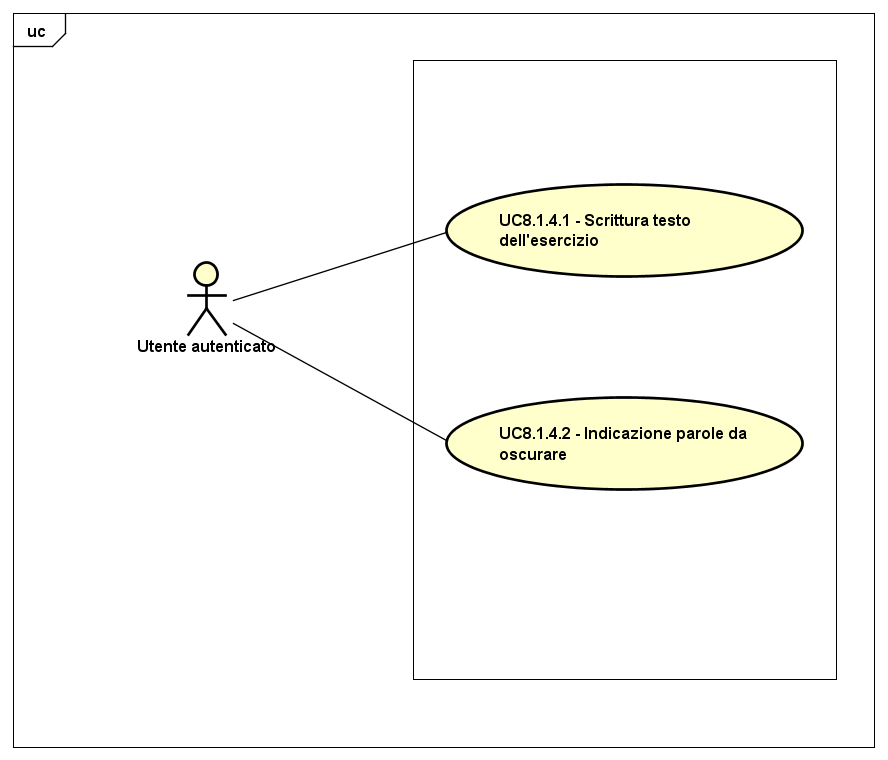
\includegraphics[scale=0.45,keepaspectratio]{UML/UC8_1_4.png}
		\caption{UC8.1.4: Creazione esercizio a riempimento di spazi vuoti}
	\end{figure}
	\FloatBarrier
	\begin{itemize}
		\item
			\textbf{Attori}: utente autenticato, utente autenticato pro;
		\item		
			\textbf{Descrizione}: l'attore può utilizzare la procedura guidata per la creazione di un esercizio a riempimento di spazi vuoti;
		\item
			\textbf{Precondizione}: il sistema presenta all'attore la procedura guidata per la creazione di un esercizio a riempimento di spazi vuoti;
		\item
			\textbf{Postcondizione}: l'attore ha creato un esercizio a riempimento di spazi vuoti;
		\item
			\textbf{Scenario principale}:
	       		\begin{enumerate}
	       			\item
	       			L'attore può inserire il testo dell'esercizio (UC8.1.4.1);
	       			\item
	       			L'attore può indicare le parole che saranno sostituite con degli spazi vuoti dal sistema (UC8.1.4.2).
	 			\end{enumerate}
	\end{itemize}
	
\subsubsection{Caso d'uso UC8.1.4.1: Scrittura testo dell'esercizio}
	\begin{itemize}
		\item
			\textbf{Attori}: utente autenticato, utente autenticato pro;
		\item		
			\textbf{Descrizione}: l'attore può inserire il testo dell'esercizio;
		\item
			\textbf{Precondizione}: il sistema presenta all'attore lo spazio destinato all'inserimento del testo dell'esercizio; 
		\item
			\textbf{Postcondizione}: l'attore ha scritto il testo dell'esercizio;
		\item
			\textbf{Scenario principale}: l'attore scrive il testo dell'esercizio.
	\end{itemize}


\subsubsection{Caso d'uso UC8.1.4.2: Indicazione parole da oscurare}
	\begin{itemize}
		\item
			\textbf{Attori}: utente autenticato, utente autenticato pro;
		\item		
			\textbf{Descrizione}: l'attore può indicare le parole che saranno sostituite con degli spazi vuoti;
		\item
			\textbf{Precondizione}: il sistema presenta all'attore lo spazio destinato all'indicazione delle parole da oscurare;  
		\item
			\textbf{Postcondizione}: l'attore ha indicato le parole che saranno sostituite con degli spazi vuoti;
		\item
			\textbf{Scenario principale}: l'attore indica le parole che verranno oscurate dal sistema.
	\end{itemize}
\subsubsection{Caso d'uso UC8.1.5: Creazione domanda di collegamento}
\label{UC8.1.5}
\begin{figure}[h]
	\centering
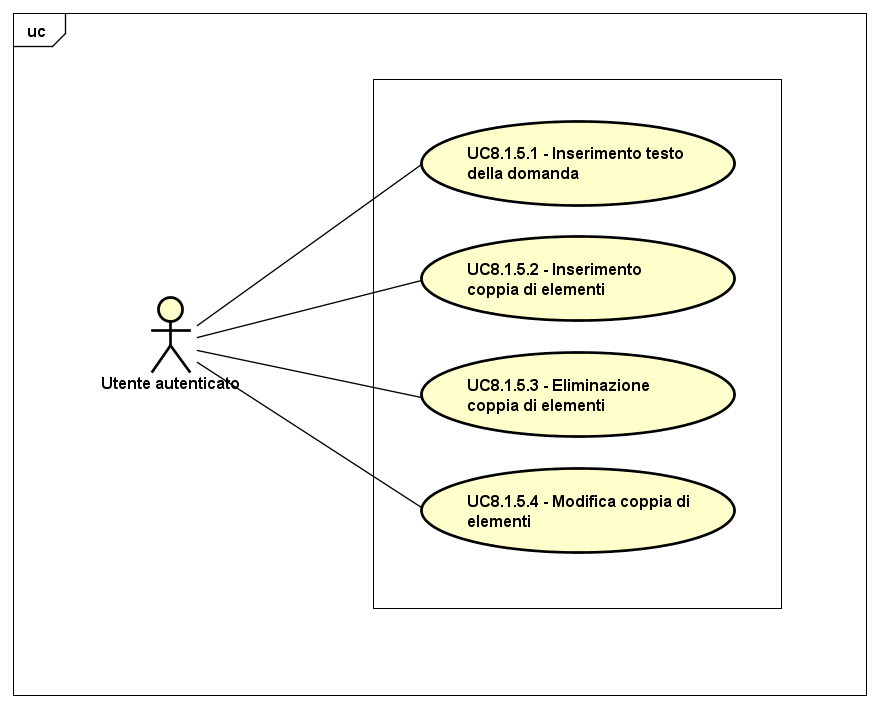
\includegraphics[scale=0.5,keepaspectratio]{UML/UC8_1_5.png}
	\caption{Caso d'uso UC8.1.5: Creazione domanda di collegamento}
\end{figure}
\FloatBarrier
\begin{itemize}
	\item \textbf{Attori}: \uau, \uaupro;
	\item \textbf{Descrizione}: l'attore può utilizzare la procedura guidata per la creazione di una domanda di collegamento; 
	\item \textbf{Precondizione}: il sistema presenta all'attore la procedura guidata per la creazione di una domanda di collegamento;
	\item \textbf{Postcondizione}: l'attore ha creato una domanda di collegamento;
	\item \textbf{Scenario principale}: 
		\begin{enumerate}
			\item L'attore può inserire il testo della domanda (UC8.1.5.1);
			\item L'attore può inserire una coppia di elementi (UC8.1.5.2);
			\item L'attore può eliminare una coppia di elementi inserita (UC8.1.5.3);
			\item L'attore può modificare una coppia di elementi inserita (UC8.1.5.4).
		\end{enumerate}
	\item \textbf{Scenari alternativi}: se non ci sono almeno due coppie presenti nella lista delle coppie l'attore deve inserire una nuova coppia di elementi.
\end{itemize}

	\subsubsection{Caso d'uso UC8.1.5.1: Inserimento testo della domanda}
	\begin{itemize}
		\item
		\textbf{Attori}: \uau, \uaupro;
		\item		
		\textbf{Descrizione}: l'attore può inserire il testo della domanda;
		\item
		\textbf{Precondizione}: il sistema presenta all'attore lo spazio destinato all'inserimento del testo della domanda;
		\item \textbf{Postcondizione}: l'attore ha inserito il testo della domanda;
		\item \textbf{Scenario principale}: l'attore inserisce il testo della domanda. 
	\end{itemize}

	\subsubsection{Caso d'uso UC8.1.5.2: Inserimento coppia di elementi}
	\begin{figure}[h]
		\centering
		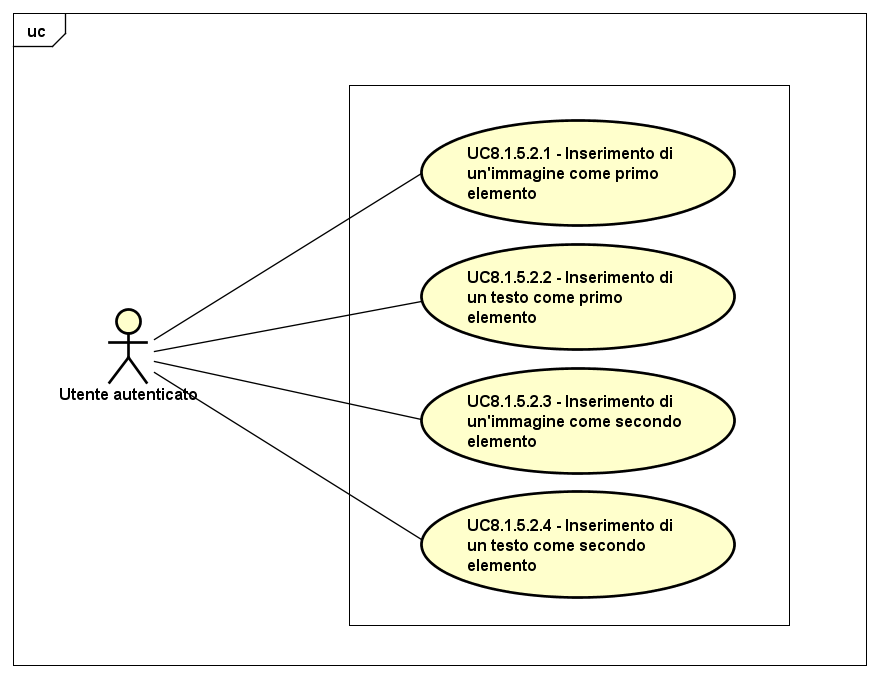
\includegraphics[scale=0.5,keepaspectratio]{UML/UC8_1_5_2.png}
		\caption{Caso d'uso UC8.1.5.2: Inserimento coppia di elementi}
	\end{figure}
	\FloatBarrier
	\begin{itemize}
		\item \textbf{Attori}: \uau, \uaupro;
		\item \textbf{Descrizione}: l'attore può inserire una coppia di elementi, sia immagini che testo o combinazioni di questi, che siano correlati tra loro in modo da indicare la soluzione della domanda; 
		\item \textbf{Precondizione}: il sistema presenta all'attore la funzionalità di inserimento di una o più coppie di elementi;
		\item \textbf{Postcondizione}: l'attore ha inserito una coppia di elementi nella lista di coppie di elementi; 
		\item \textbf{Scenario principale}: 
		\begin{enumerate}
			\item L'attore inserisce come primo elemento un'immagine (UC8.1.5.2.1);
			\item L'attore inserisce come primo elemento un testo (UC8.1.5.2.2);
			\item L'attore inserisce come secondo elemento un'immagine (UC8.1.5.2.3);
			\item L'attore inserisce come secondo elemento un testo (UC8.1.5.2.4).	
		\end{enumerate}
	\end{itemize}
	
		\subsubsection{Caso d'uso UC8.1.5.2.1: Inserimento di un'immagine come primo elemento}
		\begin{itemize}
			\item \textbf{Attori}: \uau, \uaupro;
			\item \textbf{Descrizione}: l'attore può inserire come primo elemento della coppia un'immagine;
			\item \textbf{Precondizione}: il sistema presenta all'attore lo spazio destinato all'inserimento di un'immagine come primo elemento;
			\item \textbf{Postcondizione}: l'attore ha inserito come primo elemento un'immagine;
			\item \textbf{Scenario principale}: l'attore carica un'immagine come primo elemento della coppia.
		\end{itemize}
		
		\subsubsection{Caso d'uso UC8.1.5.2.2: Inserimento di un testo come primo elemento}
		\begin{itemize}
			\item \textbf{Attori}: \uau, \uaupro;
			\item \textbf{Descrizione}: l'attore può inserire come primo elemento della coppia un testo;
			\item \textbf{Precondizione}: il sistema presenta all'attore lo spazio destinato all'inserimento di un testo come primo elemento;
			\item \textbf{Postcondizione}: l'attore ha inserito come primo elemento un testo;
			\item \textbf{Scenario principale}: l'attore inserisce del testo come primo elemento della coppia.
		\end{itemize}
		
			\subsubsection{Caso d'uso UC8.1.5.2.3: Inserimento di un'immagine come secondo elemento}
		\begin{itemize}
			\item \textbf{Attori}: \uau, \uaupro;
			\item \textbf{Descrizione}: l'attore può inserire come secondo elemento della coppia un'immagine;
			\item \textbf{Precondizione}: il sistema presenta all'attore lo spazio destinato all'inserimento di un'immagine come secondo elemento;
			\item \textbf{Postcondizione}: l'attore ha inserito come secondo elemento un'immagine;
			\item \textbf{Scenario principale}: l'attore carica un'immagine come secondo elemento della coppia.
		\end{itemize}
		
		\subsubsection{Caso d'uso UC8.1.5.2.4: Inserimento di un testo come secondo elemento}
		\begin{itemize}
			\item \textbf{Attori}: \uau, \uaupro;
			\item \textbf{Descrizione}: l'attore può inserire come secondo elemento della coppia un testo;
			\item \textbf{Precondizione}: il sistema presenta all'attore lo spazio destinato all'inserimento di un testo come secondo elemento;
			\item \textbf{Postcondizione}: l'attore ha inserito come secondo elemento un testo;
			\item \textbf{Scenario principale}: l'attore inserisce del testo come secondo elemento della coppia.
		\end{itemize}
	
	\subsubsection{Caso d'uso UC8.1.5.3: Eliminazione coppia di elementi}
	\begin{figure}[h]
		\centering
		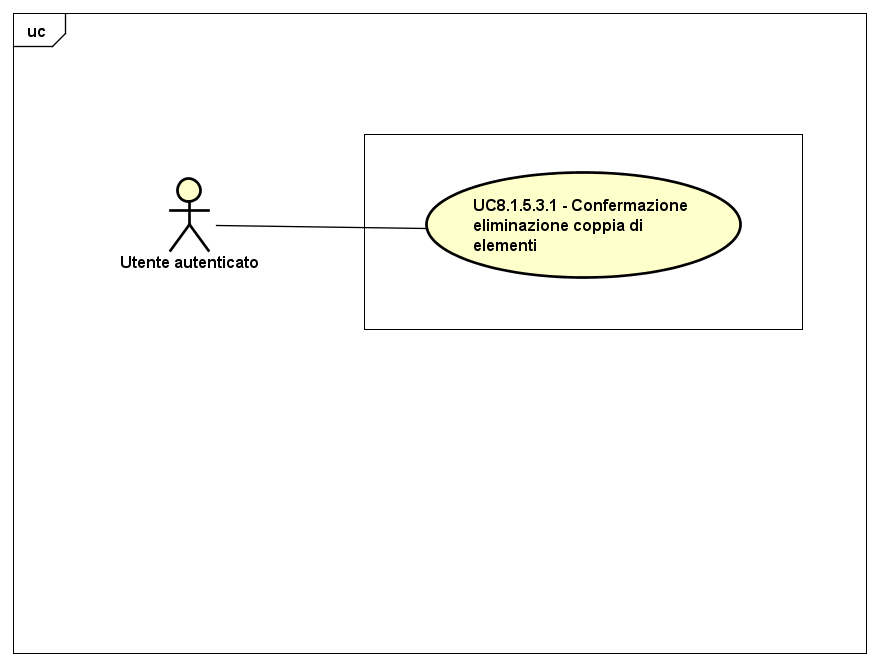
\includegraphics[scale=0.5,keepaspectratio]{UML/UC8_1_5_3.png}
		\caption{Caso d'uso UC8.1.5.3: Eliminazione coppia di elementi}
	\end{figure}
	\FloatBarrier
	\begin{itemize}
		\item \textbf{Attori}: \uau, \uaupro;
		\item \textbf{Descrizione}: l'attore può rimuovere una coppia di elementi dalla lista di coppie di elementi;
		\item \textbf{Precondizione}: il sistema presenta all'attore la funzionalità di eliminare una coppia di elementi;
		\item \textbf{Postcondizione}: l'attore ha eliminato una coppia di elementi dalla lista delle coppie di elementi;
		\item \textbf{Scenario principale}: l'attore può confermare l'eliminazione di una coppia di elementi (UC8.1.5.3.1);	
		\item \textbf{Scenari alternativi}: l'attore annulla l'operazione tornando alla schermata precedente.
	\end{itemize}

		\subsubsection{Caso d'uso UC8.1.5.3.1: Conferma eliminazione coppia di elementi}
		\begin{itemize}
			\item \textbf{Attori}: \uau, \uaupro;
			\item \textbf{Descrizione}: l'attore può confermare la rimozione di una coppia di elementi;
			\item \textbf{Precondizione}: il sistema presenta all'attore la funzionalità di confermare l'eliminazione di una coppia di elementi;
			\item \textbf{Postcondizione}: l'attore ha confermato l'eliminazione della coppia di elementi;
			\item \textbf{Scenario principale}: l'attore conferma la rimozione della coppia di elementi.
		\end{itemize}

	\subsubsection{Caso d'uso UC8.1.5.4: Modifica coppia di elementi}
	\label{UC8.1.5.4}
	\begin{figure}[h]
		\centering
		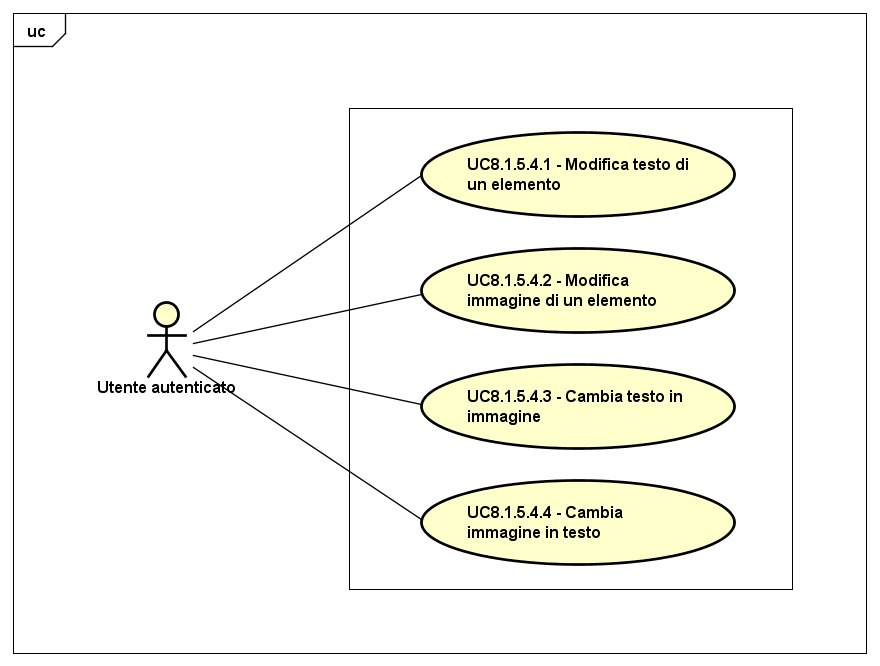
\includegraphics[scale=0.5,keepaspectratio]{UML/UC8_1_5_4.png}
		\caption{Caso d'uso UC8.1.5.4: Modifica coppia di elementi}
	\end{figure}
	\FloatBarrier
	\begin{itemize}
		\item \textbf{Attori}: \uau, \uaupro;
		\item \textbf{Descrizione}: l'attore può modificare una coppia di elementi presente nella lista di coppie di elementi;
		\item \textbf{Precondizione}: il sistema presenta all'attore la funzionalità di modificare una coppia di elementi;
		\item \textbf{Postcondizione}: l'attore ha modificato una coppia di elementi presente nella lista di coppie di elementi; 
		\item \textbf{Scenario principale}: 
		\begin{enumerate}
			\item L'attore può modificare un elemento cambiandone il testo (UC8.1.5.4.1);
			\item L'attore può modificare un elemento cambiandone l'immagine (UC8.1.5.4.2);
			\item L'attore può modificare un elemento facendolo passare da testo ad immagine \\(UC8.1.5.4.3);
			\item L'attore può modificare un elemento facendolo passare da immagine a testo \\(UC8.1.5.4.4).	
		\end{enumerate}
	\end{itemize}
	
		\subsubsection{Caso d'uso UC8.1.5.4.1: Modifica testo di un elemento}
		\begin{itemize}
			\item \textbf{Attori}: \uau, \uaupro;
			\item \textbf{Descrizione}: l'attore può modificare il testo di un elemento;
			\item \textbf{Precondizione}: il sistema presenta all'attore la funzionalità di modificare il testo di un elemento;
			\item \textbf{Postcondizione}: l'attore ha modificato il testo di un elemento;
			\item \textbf{Scenario principale}: l'attore modifica il testo di un elemento.  
		\end{itemize}
		
		\subsubsection{Caso d'uso UC8.1.5.4.2: Modifica immagine di un elemento}
		\begin{itemize}
			\item \textbf{Attori}: \uau, \uaupro;
			\item \textbf{Descrizione}: l'attore può caricare un'altra immagine per un elemento;
			\item \textbf{Precondizione}: il sistema presenta all'attore la funzionalità di modificare l'immagine di un elemento; 
			\item \textbf{Postcondizione}: l'attore ha inserito un'altra immagine per un elemento;
			\item \textbf{Scenario principale}: l'attore carica un'altra immagine per un elemento.
		\end{itemize}
		
		\subsubsection{Caso d'uso UC8.1.5.4.3: Cambia testo in immagine}
		\begin{itemize}
			\item \textbf{Attori}: \uau, \uaupro;
			\item \textbf{Descrizione}: l'attore può modificare un elemento facendolo diventare un'immagine al posto di un testo;
			\item \textbf{Precondizione}: il sistema presenta all'attore la funzionalità di modificare un elemento facendolo diventare un'immagine al posto di un testo;
			\item \textbf{Postcondizione}: l'attore ha fatto diventare un'immagine un elemento che prima era un testo;
			\item \textbf{Scenario principale}: l'attore inserisce un'immagine come modifica dell'elemento.  
		\end{itemize}
		
		\subsubsection{Caso d'uso UC8.1.5.4.4: Cambia immagine in testo}
		\begin{itemize}
			\item \textbf{Attori}: \uau, \uaupro;
			\item \textbf{Descrizione}: l'attore può modificare un elemento facendolo diventare un testo al posto di un'immagine;
			\item \textbf{Precondizione}: il sistema presenta all'attore la funzionalità di modificare un elemento facendolo diventare un testo al posto di un'immagine;
			\item \textbf{Postcondizione}: l'attore ha fatto diventare un testo un elemento che prima era un'immagine;
			\item \textbf{Scenario principale}: l'attore inserisce del testo come modifica dell'elemento.  
		\end{itemize}
		

\subsubsection{Caso d'uso UC8.1.6: Creazione domanda a ordinamento di immagini}
\label{UC8.1.6}
	\begin{figure}[ht]
		\centering
			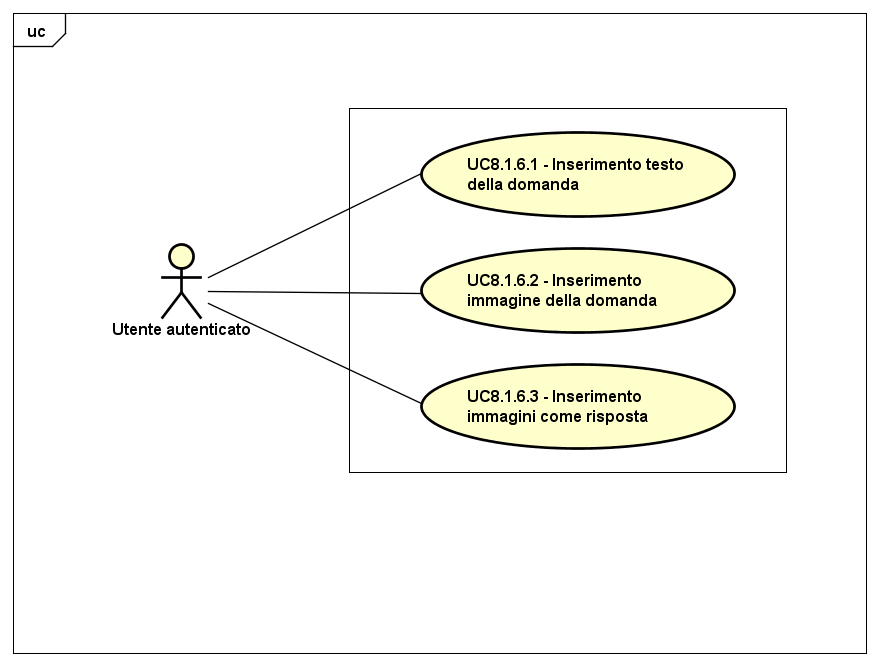
\includegraphics[scale=0.45,keepaspectratio]{UML/UC8_1_6.png}
		\caption{UC8.1.6: Creazione domanda a ordinamento di immagini}
	\end{figure}
	\FloatBarrier
\begin{itemize}
	\item\textbf{Attori}: utente autenticato, utente autenticato pro;
	\item\textbf{Descrizione}: l'attore può utilizzare la procedura guidata per la creazione di una domanda a ordinamento di immagini;
	\item\textbf{Precondizione}: il sistema presenta all'attore la procedura guidata per la creazione di una domanda a ordinamento di immagini; 
	\item \textbf{Postcondizione}: l'attore ha creato una domanda a ordinamento di immagini;
	\item\textbf{Scenario principale}:
	\begin{itemize}
		\item L'attore può inserire il testo della domanda (UC8.1.6.1);
		\item L'attore può inserire un'immagine relativa al testo della domanda (UC8.1.6.2);
		\item L'attore può inserire le immagini della sequenza che costituirà la risposta (UC8.1.6.3).
	\end{itemize}
\end{itemize}

\subsubsection{Caso d'uso UC8.1.6.1: Inserimento testo della domanda}
\begin{itemize}
	\item\textbf{Attori}: utente autenticato, utente autenticato pro;
	\item\textbf{Descrizione}: l'attore può inserire il testo della domanda;
	\item\textbf{Precondizione}: il sistema presenta all'attore lo spazio destinato all'inserimento del testo della domanda;
	\item \textbf{Postcondizione}: l'attore ha inserito il testo della domanda;
	\item\textbf{Scenario principale}: l'attore inserisce il testo della domanda. 
\end{itemize}

\subsubsection{Caso d'uso UC8.1.6.2: Inserimento immagine della domanda}
\begin{itemize}
	\item\textbf{Attori}: utente autenticato, utente autenticato pro;
	\item\textbf{Descrizione}: l'attore può inserire un'immagine relativa al testo della domanda;
	\item\textbf{Precondizione}: il sistema presenta all'attore la funzionalità di inserire un'immagine;
	\item \textbf{Postcondizione}: l'attore ha inserito un'immagine relativa al testo della domanda;
	\item\textbf{Scenario principale}: l'attore inserisce un'immagine.
\end{itemize}

\subsubsection{Caso d'uso UC8.1.6.3: Inserimento immagini come risposta}
\begin{itemize}
	\item\textbf{Attori}: utente autenticato, utente autenticato pro;
	\item\textbf{Descrizione}: l'attore può inserire le immagini che costituiscono la risposta alla domanda e indicare poi la soluzione di questa mettendole nell'ordine corretto;
	\item\textbf{Precondizione}: il sistema presenta all'attore la funzionalità di inserire due o più immagini come risposta; 
	\item \textbf{Postcondizione}: l'attore ha inserito le immagini che costituiscono la risposta alla domanda e le ha ordinate in base alla soluzione di questa;
	\item\textbf{Scenario principale}: l'attore inserisce una o più immagini come risposta.
\end{itemize}


\subsubsection{Caso d'uso UC8.1.7: Creazione domanda di collegamento}
\label{UC8.1.7}
\begin{figure}[h]
	\centering
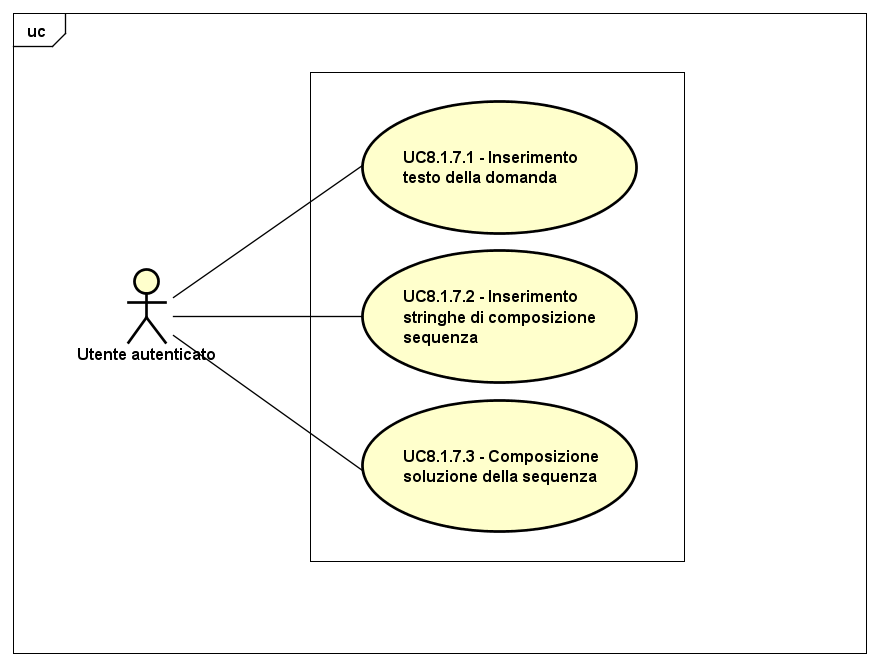
\includegraphics[scale=0.5,keepaspectratio]{UML/UC8_1_7.png}
	\caption{Caso d'uso UC8.1.7: Creazione domanda di collegamento}
\end{figure}
\FloatBarrier
\begin{itemize}
	\item \textbf{Attori}: \uau, \uaupro;
	\item \textbf{Descrizione}: l'attore può utilizzare la procedura guidata per la creazione di una domanda di collegamento; 
	\item \textbf{Precondizione}: il sistema presenta all'attore la procedura guidata per la creazione di una domanda di collegamento;
	\item \textbf{Postcondizione}: l'attore ha creato una domanda di collegamento;
	\item \textbf{Scenario principale}: 
		\begin{enumerate}
			\item L'attore può inserire il testo della domanda (UC8.1.7.1);
			\item L'attore può inserire una coppia di elementi (UC8.1.7.2);
			\item L'attore può eliminare una coppia di elementi inserita (UC8.1.7.3);
			\item L'attore può modificare una coppia di elementi inserita (UC8.1.7.4).
		\end{enumerate}
	\item \textbf{Scenari alternativi}: se non ci sono almeno due coppie presenti nella lista delle coppie l'attore deve inserire una nuova coppia di elementi.
\end{itemize}

	\subsubsection{Caso d'uso UC8.1.7.1: Inserimento testo della domanda}
	\begin{itemize}
		\item
		\textbf{Attori}: \uau, \uaupro;
		\item		
		\textbf{Descrizione}: l'attore può inserire il testo della domanda;
		\item
		\textbf{Precondizione}: il sistema presenta all'attore lo spazio destinato all'inserimento del testo della domanda;
		\item \textbf{Postcondizione}: l'attore ha inserito il testo della domanda;
		\item \textbf{Scenario principale}: l'attore inserisce il testo della domanda. 
	\end{itemize}

	\subsubsection{Caso d'uso UC8.1.7.2: Inserimento coppia di elementi}
	\begin{figure}[h]
		\centering
		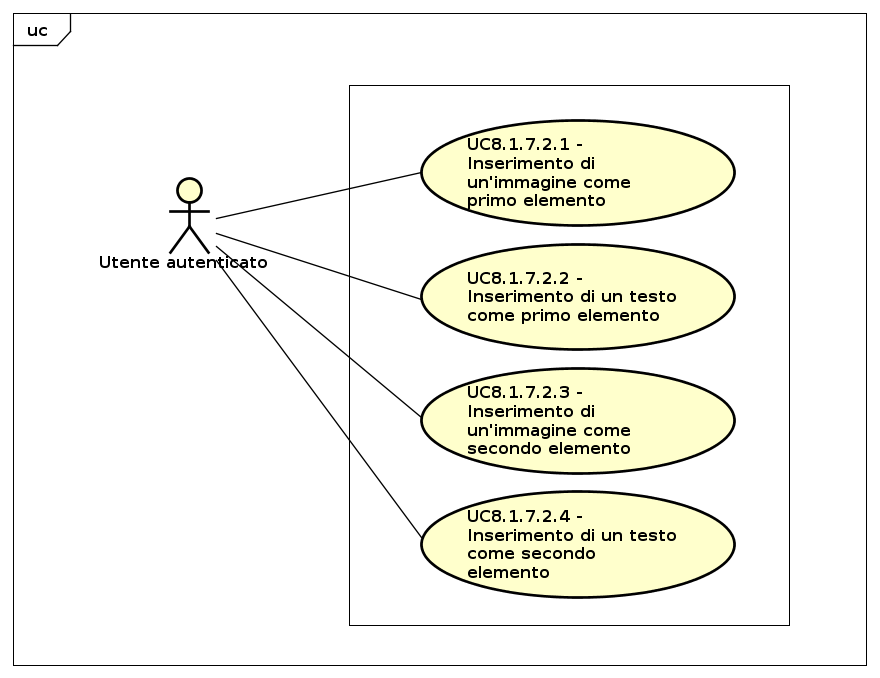
\includegraphics[scale=0.5,keepaspectratio]{UML/UC8_1_7_2.png}
		\caption{Caso d'uso UC8.1.7.2: Inserimento coppia di elementi}
	\end{figure}
	\FloatBarrier
	\begin{itemize}
		\item \textbf{Attori}: \uau, \uaupro;
		\item \textbf{Descrizione}: l'attore può inserire una coppia di elementi, sia immagini che testo o combinazioni di questi, che siano correlati tra loro in modo da indicare la soluzione della domanda; 
		\item \textbf{Precondizione}: il sistema presenta all'attore la funzionalità di inserimento di una o più coppie di elementi;
		\item \textbf{Postcondizione}: l'attore ha inserito una coppia di elementi nella lista di coppie di elementi; 
		\item \textbf{Scenario principale}: 
		\begin{enumerate}
			\item L'attore inserisce come primo elemento un'immagine (UC8.1.7.2.1);
			\item L'attore inserisce come primo elemento un testo (UC8.1.7.2.2);
			\item L'attore inserisce come secondo elemento un'immagine (UC8.1.7.2.3);
			\item L'attore inserisce come secondo elemento un testo (UC8.1.7.2.4).	
		\end{enumerate}
	\end{itemize}
	
		\subsubsection{Caso d'uso UC8.1.7.2.1: Inserimento di un'immagine come primo elemento}
		\begin{itemize}
			\item \textbf{Attori}: \uau, \uaupro;
			\item \textbf{Descrizione}: l'attore può inserire come primo elemento della coppia un'immagine;
			\item \textbf{Precondizione}: il sistema presenta all'attore lo spazio destinato all'inserimento di un'immagine come primo elemento;
			\item \textbf{Postcondizione}: l'attore ha inserito come primo elemento un'immagine;
			\item \textbf{Scenario principale}: l'attore carica un'immagine come primo elemento della coppia.
		\end{itemize}
		
		\subsubsection{Caso d'uso UC8.1.7.2.2: Inserimento di un testo come primo elemento}
		\begin{itemize}
			\item \textbf{Attori}: \uau, \uaupro;
			\item \textbf{Descrizione}: l'attore può inserire come primo elemento della coppia un testo;
			\item \textbf{Precondizione}: il sistema presenta all'attore lo spazio destinato all'inserimento di un testo come primo elemento;
			\item \textbf{Postcondizione}: l'attore ha inserito come primo elemento un testo;
			\item \textbf{Scenario principale}: l'attore inserisce del testo come primo elemento della coppia.
		\end{itemize}
		
			\subsubsection{Caso d'uso UC8.1.7.2.3: Inserimento di un'immagine come secondo elemento}
		\begin{itemize}
			\item \textbf{Attori}: \uau, \uaupro;
			\item \textbf{Descrizione}: l'attore può inserire come secondo elemento della coppia un'immagine;
			\item \textbf{Precondizione}: il sistema presenta all'attore lo spazio destinato all'inserimento di un'immagine come secondo elemento;
			\item \textbf{Postcondizione}: l'attore ha inserito come secondo elemento un'immagine;
			\item \textbf{Scenario principale}: l'attore carica un'immagine come secondo elemento della coppia.
		\end{itemize}
		
		\subsubsection{Caso d'uso UC8.1.7.2.4: Inserimento di un testo come secondo elemento}
		\begin{itemize}
			\item \textbf{Attori}: \uau, \uaupro;
			\item \textbf{Descrizione}: l'attore può inserire come secondo elemento della coppia un testo;
			\item \textbf{Precondizione}: il sistema presenta all'attore lo spazio destinato all'inserimento di un testo come secondo elemento;
			\item \textbf{Postcondizione}: l'attore ha inserito come secondo elemento un testo;
			\item \textbf{Scenario principale}: l'attore inserisce del testo come secondo elemento della coppia.
		\end{itemize}
	
	\subsubsection{Caso d'uso UC8.1.7.3: Eliminazione coppia di elementi}
	\begin{figure}[h]
		\centering
		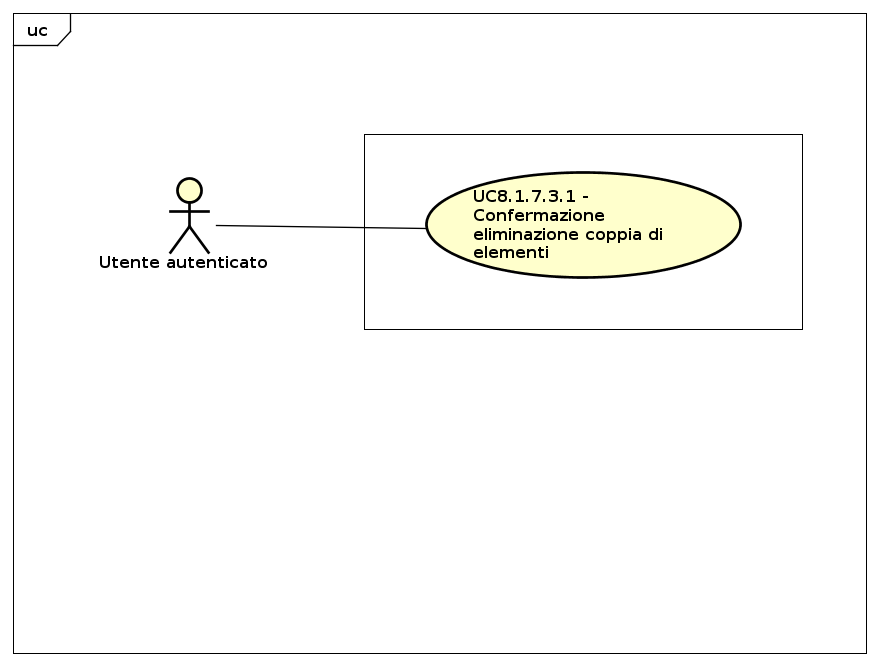
\includegraphics[scale=0.5,keepaspectratio]{UML/UC8_1_7_3.png}
		\caption{Caso d'uso UC8.1.7.3: Eliminazione coppia di elementi}
	\end{figure}
	\FloatBarrier
	\begin{itemize}
		\item \textbf{Attori}: \uau, \uaupro;
		\item \textbf{Descrizione}: l'attore può rimuovere una coppia di elementi dalla lista di coppie di elementi;
		\item \textbf{Precondizione}: il sistema presenta all'attore la funzionalità di eliminare una coppia di elementi;
		\item \textbf{Postcondizione}: l'attore ha eliminato una coppia di elementi dalla lista delle coppie di elementi;
		\item \textbf{Scenario principale}: l'attore può confermare l'eliminazione di una coppia di elementi (UC8.1.7.3.1);	
		\item \textbf{Scenari alternativi}: l'attore annulla l'operazione tornando alla schermata precedente.
	\end{itemize}

		\subsubsection{Caso d'uso UC8.1.7.3.1: Conferma eliminazione coppia di elementi}
		\begin{itemize}
			\item \textbf{Attori}: \uau, \uaupro;
			\item \textbf{Descrizione}: l'attore può confermare la rimozione di una coppia di elementi;
			\item \textbf{Precondizione}: il sistema presenta all'attore la funzionalità di confermare l'eliminazione di una coppia di elementi;
			\item \textbf{Postcondizione}: l'attore ha confermato l'eliminazione della coppia di elementi;
			\item \textbf{Scenario principale}: l'attore conferma la rimozione della coppia di elementi.
		\end{itemize}

	\subsubsection{Caso d'uso UC8.1.7.4: Modifica coppia di elementi}
	\label{UC8.1.7.4}
	\begin{figure}[h]
		\centering
		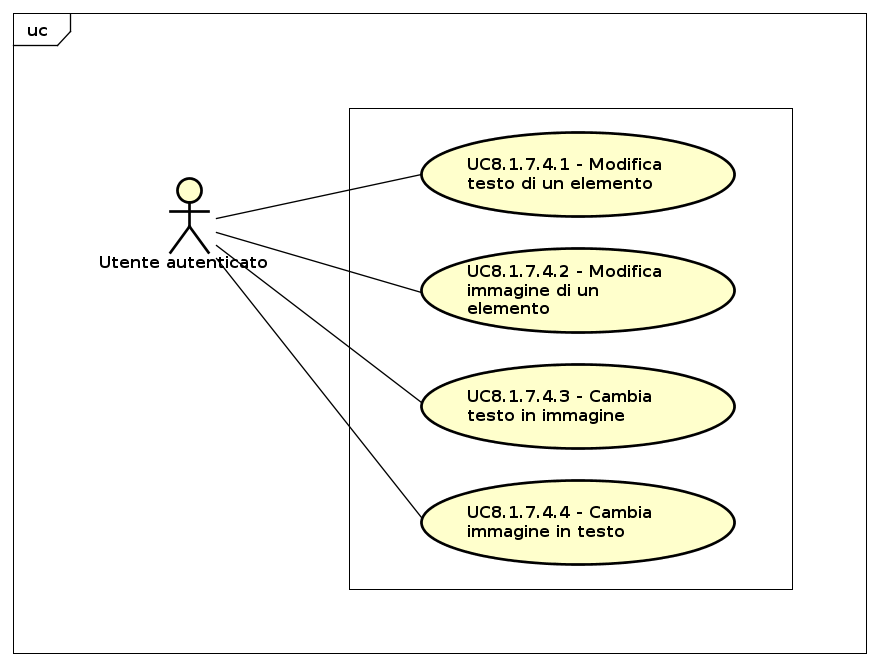
\includegraphics[scale=0.5,keepaspectratio]{UML/UC8_1_7_4.png}
		\caption{Caso d'uso UC8.1.7.4: Modifica coppia di elementi}
	\end{figure}
	\FloatBarrier
	\begin{itemize}
		\item \textbf{Attori}: \uau, \uaupro;
		\item \textbf{Descrizione}: l'attore può modificare una coppia di elementi presente nella lista di coppie di elementi;
		\item \textbf{Precondizione}: il sistema presenta all'attore la funzionalità di modificare una coppia di elementi;
		\item \textbf{Postcondizione}: l'attore ha modificato una coppia di elementi presente nella lista di coppie di elementi; 
		\item \textbf{Scenario principale}: 
		\begin{enumerate}
			\item L'attore può modificare un elemento cambiandone il testo (UC8.1.7.4.1);
			\item L'attore può modificare un elemento cambiandone l'immagine (UC8.1.7.4.2);
			\item L'attore può modificare un elemento facendolo passare da testo ad immagine \\(UC8.1.7.4.3);
			\item L'attore può modificare un elemento facendolo passare da immagine a testo \\(UC8.1.7.4.4).	
		\end{enumerate}
	\end{itemize}
	
		\subsubsection{Caso d'uso UC8.1.7.4.1: Modifica testo di un elemento}
		\begin{itemize}
			\item \textbf{Attori}: \uau, \uaupro;
			\item \textbf{Descrizione}: l'attore può modificare il testo di un elemento;
			\item \textbf{Precondizione}: il sistema presenta all'attore la funzionalità di modificare il testo di un elemento;
			\item \textbf{Postcondizione}: l'attore ha modificato il testo di un elemento;
			\item \textbf{Scenario principale}: l'attore modifica il testo di un elemento.  
		\end{itemize}
		
		\subsubsection{Caso d'uso UC8.1.7.4.2: Modifica immagine di un elemento}
		\begin{itemize}
			\item \textbf{Attori}: \uau, \uaupro;
			\item \textbf{Descrizione}: l'attore può caricare un'altra immagine per un elemento;
			\item \textbf{Precondizione}: il sistema presenta all'attore la funzionalità di modificare l'immagine di un elemento; 
			\item \textbf{Postcondizione}: l'attore ha inserito un'altra immagine per un elemento;
			\item \textbf{Scenario principale}: l'attore carica un'altra immagine per un elemento.
		\end{itemize}
		
		\subsubsection{Caso d'uso UC8.1.7.4.3: Cambia testo in immagine}
		\begin{itemize}
			\item \textbf{Attori}: \uau, \uaupro;
			\item \textbf{Descrizione}: l'attore può modificare un elemento facendolo diventare un'immagine al posto di un testo;
			\item \textbf{Precondizione}: il sistema presenta all'attore la funzionalità di modificare un elemento facendolo diventare un'immagine al posto di un testo;
			\item \textbf{Postcondizione}: l'attore ha fatto diventare un'immagine un elemento che prima era un testo;
			\item \textbf{Scenario principale}: l'attore inserisce un'immagine come modifica dell'elemento.  
		\end{itemize}
		
		\subsubsection{Caso d'uso UC8.1.7.4.4: Cambia immagine in testo}
		\begin{itemize}
			\item \textbf{Attori}: \uau, \uaupro;
			\item \textbf{Descrizione}: l'attore può modificare un elemento facendolo diventare un testo al posto di un'immagine;
			\item \textbf{Precondizione}: il sistema presenta all'attore la funzionalità di modificare un elemento facendolo diventare un testo al posto di un'immagine;
			\item \textbf{Postcondizione}: l'attore ha fatto diventare un testo un elemento che prima era un'immagine;
			\item \textbf{Scenario principale}: l'attore inserisce del testo come modifica dell'elemento.  
		\end{itemize}
		

\subsubsection{Caso d'uso UC8.1.8: Creazione domanda con area cliccabile nell'immagine}
\label{UC8.1.8}
\begin{figure}[ht]
	\centering
	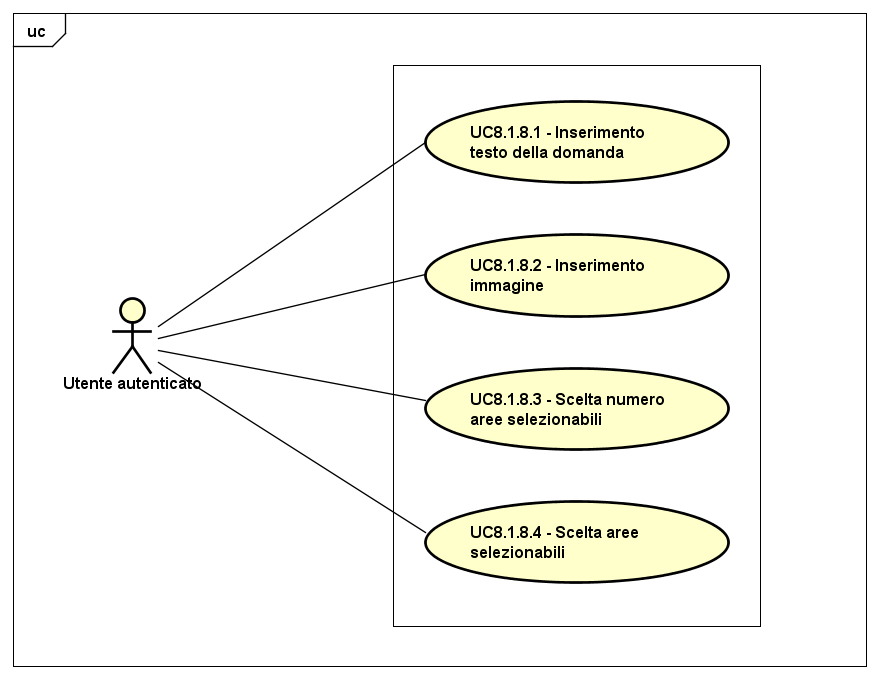
\includegraphics[scale=0.5,keepaspectratio]{UML/UC8_1_8.png}
	\caption{UC8.1.8: Creazione domanda con area cliccabile nell'immagine}
\end{figure}
\FloatBarrier
\begin{itemize}
	\item \textbf{Attori}: utente autenticato, utente autenticato pro;
	\item \textbf{Descrizione}: l'attore ha selezionato la funzionalità di creazione di una domanda la cui risposta è selezionabile all'interno di aree cliccabili in un'immagine;
	\item \textbf{Precondizione}: il sistema presenta all'attore la procedura guidata per la creazione di una domanda con area cliccabile nell'immagine;
	\item \textbf{Postcondizione}: l'attore ha creato una domanda con area cliccabile nell'immagine;
	\item \textbf{Scenario principale}:
		\begin{enumerate}
	       	\item L'attore può inserire il testo della domanda (UC8.1.8.1);
	        \item L'attore può inserire un'immagine relativa al testo della domanda (UC8.1.8.2);
		\item L'attore può scegliere quante aree saranno selezionabili all'interno dell'immagine \\(UC8.1.8.3);
		\item L'attore può scegliere quali aree saranno selezionabili all'interno dell'immagine \\(UC8.1.8.4).
	 	\end{enumerate}
\end{itemize}

\subsubsection{Caso d'uso UC8.1.8.1: Inserimento testo della domanda}
\begin{itemize}
	\item \textbf{Attori}: utente autenticato, utente autenticato pro;
	\item \textbf{Descrizione}: l'attore può inserire il testo della domanda che vuole creare;
	\item \textbf{Precondizione}: il sistema presenta all'attore lo spazio destinato all'inserimento del testo della domanda;
	\item \textbf{Postcondizione}: l'attore ha inserito il testo della domanda;
	\item \textbf{Scenario principale}: l'attore inserisce il testo della domanda. 
\end{itemize}

\subsubsection{Caso d'uso UC8.1.8.2: Inserimento immagine}
\begin{itemize}
	\item \textbf{Attori}: utente autenticato, utente autenticato pro;
	\item \textbf{Descrizione}: l'attore può inserire un'immagine relativa al testo della domanda;
	\item \textbf{Precondizione}: il sistema presenta all'attore la funzionalità di inserire un'immagine;
	\item \textbf{Postcondizione}: l'attore ha inserito un'immagine relativa al testo della domanda;
	\item \textbf{Scenario principale}: l'attore può eliminare l'immagine inserita (UC8.1.3.7.2.1).			
	\end{itemize}

\subsubsection{Caso d'uso UC8.1.8.3: Scelta numero aree selezionabili}
\begin{itemize}
	\item \textbf{Attori}: utente autenticato, utente autenticato pro;
	\item \textbf{Descrizione}: l'attore può scegliere il numero di aree selezionabili all'interno dell'immagine;
	\item \textbf{Precondizione}: il sistema presenta all'attore la funzionalità di scegliere il numero di aree selezionabili all'interno dell'immagine; 	
	\item \textbf{Postcondizione}: l'attore ha scelto il numero di aree selezionabili all'interno dell'immagine;
	\item \textbf{Scenario principale}: l'attore sceglie il numero di aree selezionabili all'interno dell'immagine. 	
\end{itemize}

\subsubsection{Caso d'uso UC8.1.8.4: Scelta aree selezionabili}
\begin{itemize}
	\item \textbf{Attori}: utente autenticato, utente autenticato pro;
	\item \textbf{Descrizione}: l'attore ha la possibilità di scegliere dove inserire le aree selezionabili all'interno dell'immagine;
	\item \textbf{Precondizione}: il sistema presenta all'attore la funzionalità di scegliere dove inserire le aree selezionabili all'interno dell'immagine; 	
	\item \textbf{Postcondizione}: l'attore ha scelto dove inserire le aree selezionabili all'interno dell'immagine;
	\item \textbf{Scenario principale}: l'attore sceglie dove inserire le aree selezionabili all'interno dell'immagine. 	
\end{itemize}




	\subsubsection{Caso d'uso UC8.1.9: Conferma creazione}
	\begin{itemize}
		\item
			\textbf{Attori}: utente autenticato, utente autenticato pro;
		\item
			\textbf{Descrizione}: l'attore può confermare la creazione della domanda effettuata con la procedura guidata;
		\item		
			\textbf{Precondizione}: il sistema presenta la funzionalità di confermare la creazione di una domanda tramite un \textit{wizard\ped{G}};
		\item
			\textbf{Postcondizione}: l'attore ha creato una domanda;
		\item
			\textbf{Scenario principale}: l'attore conferma la creazione della domanda;		
		\item
	 		\textbf{Scenari alternativi}: l'attore annulla la creazione della domanda.
					
	\end{itemize}	
	
	\subsubsection{Caso d'uso UC8.1.10: Visualizzazione errore creazione domanda}
	\begin{itemize}
		\item
			\textbf{Attori}: utente autenticato, utente autenticato pro;
		\item
			\textbf{Descrizione}: l'attore può visualizzare un messaggio d'errore nel caso si fossero verificati uno o più scenari alternativi durante la creazione della domanda;
		\item		
			\textbf{Precondizione}: il sistema ha ricevuto dei dati errati per la creazione della domanda;
		\item
			\textbf{Postcondizione}: il sistema mostra un messaggio d'errore;
		\item
			\textbf{Scenario principale}: l'attore visualizza un messaggio d'errore;	
	\end{itemize}	


	\subsubsection{Caso d'uso UC8.2: Modifica domanda esistente tramite procedura guidata}
	\label{UC8.2}
	\begin{figure}[h]
		\centering
			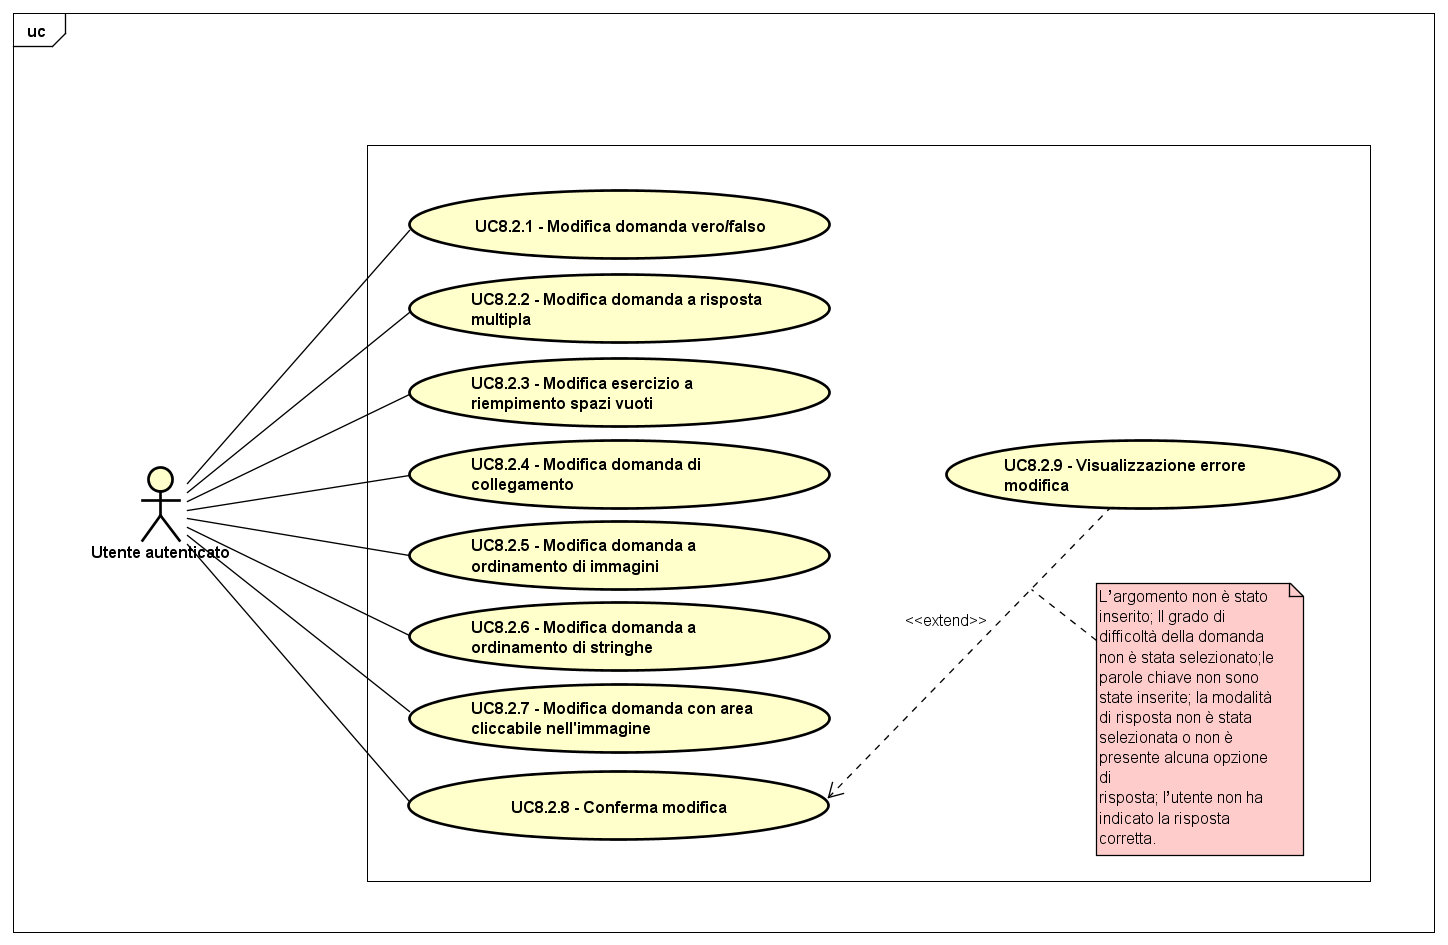
\includegraphics[scale=0.41,keepaspectratio]{UML/UC8_2.png}
		\caption{UC8.2: Modifica domanda esistente tramite procedura guidata}
	\end{figure}
	\FloatBarrier
	\begin{itemize}
		\item
			\textbf{Attori}: utente autenticato, utente autenticato pro;
		\item		
			\textbf{Descrizione}: l'attore può modificare, tramite procedura guidata, una domanda che aveva creato precedentemente;
		\item
			\textbf{Precondizione}: il sistema visualizza la schermata di modifica di una domanda;
		\item
			\textbf{Postcondizione}: l'attore modifica una domanda;
		\item
			\textbf{Scenario principale}:
				\begin{enumerate} 
					\item
					L'attore può richiamare il \textit{wizard\ped{G}} per modificare una domanda vero/falso (UC8.2.1);
					\item
					L'attore può richiamare il \textit{wizard\ped{G}} per modificare una domanda a risposta multipla (UC8.2.2);
					\item
					L'attore può richiamare il \textit{wizard\ped{G}} per modificare un esercizio a riempimento di spazi vuoti (UC8.2.3);
					\item
					L'attore può richiamare il \textit{wizard\ped{G}} per modificare una domanda di collegamento (UC8.2.4);
					\item
					L'attore può richiamare il \textit{wizard\ped{G}} per modificare una domanda a ordinamento di immagini (UC8.2.5);
					\item
					L'attore può richiamare il \textit{wizard\ped{G}} per modificare una domanda a ordinamento di stringhe (UC8.2.6);
					\item
					L'attore può richiamare il \textit{wizard\ped{G}} per modificare una domanda con area cliccabile nell'immagine (UC8.2.7).
					\item
					L'attore può confermare le modifiche apportate (UC8.2.8);
				\end{enumerate}	
	 	\item
			\textbf{Estensioni}: l'attore visualizza un messaggio d'errore relativo alla modifica della domanda (UC8.2.9);
	\end{itemize}
	
%inclusione file latex wizard
\subsubsection{Caso d'uso UC8.2.1: Modifica domanda vero/falso}
	\label{UC8.2.1}
	\begin{figure}[ht]
		\centering
			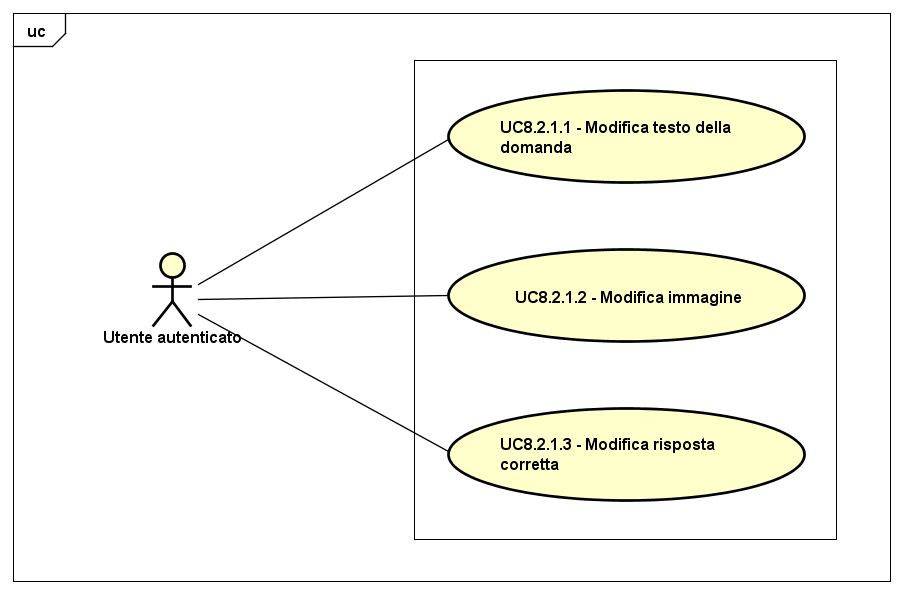
\includegraphics[scale=0.45,keepaspectratio]{UML/UC8_2_1.png}
		\caption{UC8.2.1: Modifica domanda vero/falso}
	\end{figure}
	\FloatBarrier
	\begin{itemize}
		\item
			\textbf{Attori}: utente autenticato, utente autenticato pro;
		\item		
			\textbf{Descrizione}: l'attore può utilizzare la procedura guidata per la modifica di una domanda vero/falso;
		\item
			\textbf{Precondizione}: il sistema ha ricevuto dall'attore la domanda da modificare;  
		\item
			\textbf{Postcondizione}: l'attore ha modificato una domanda vero/falso;
		\item
			\textbf{Scenario principale}:
	       		\begin{enumerate}
	       			\item
	       			L'attore può modificare il testo della domanda (UC8.2.1.1);
	       			\item
	       			L'attore può modificare l'immagine relativa al testo della domanda (UC8.2.1.2);
					\item
					L'attore può modificare la risposta corretta (UC8.2.1.3).
	 			\end{enumerate}
	\end{itemize}
	
\subsubsection{Caso d'uso UC8.2.1.1: Modifica testo della domanda}
	\begin{itemize}
		\item
			\textbf{Attori}: utente autenticato, utente autenticato pro;
		\item		
			\textbf{Descrizione}: l'attore può modificare il testo della domanda;
		\item
			\textbf{Precondizione}: il sistema mostra la funzionalità di modifica di una domanda \\vero/falso; 
		\item
			\textbf{Postcondizione}: l'attore ha modificato il testo della domanda;
		\item
			\textbf{Scenario principale}: l'attore modifica il testo della domanda. 
	\end{itemize}
	
\subsubsection{Caso d'uso UC8.2.1.2: Modifica immagine}
	\begin{itemize}
		\item
			\textbf{Attori}: utente autenticato, utente autenticato pro;
		\item		
			\textbf{Descrizione}: l'attore può modificare l'immagine relativa al testo della domanda;
		\item
			\textbf{Precondizione}: il sistema mostra la funzionalità di modifica di una domanda \\vero/falso; 
		\item
			\textbf{Postcondizione}: l'attore ha modificato l'immagine relativa al testo della domanda;
		\item
			\textbf{Scenario principale}: l'attore modifica l'immagine relativa al testo della domanda. 	
	\end{itemize}
	
\subsubsection{Caso d'uso UC8.2.1.3: Modifica risposta corretta}
	\begin{itemize}
		\item
			\textbf{Attori}: utente autenticato, utente autenticato pro;
		\item		
			\textbf{Descrizione}: l'attore può modificare la selezione della risposta corretta;
		\item
			\textbf{Precondizione}: il sistema mostra la funzionalità di modifica di una domanda \\vero/falso; 
		\item
			\textbf{Postcondizione}: l'attore ha modificato la selezione della risposta corretta;
		\item
			\textbf{Scenario principale}: l'attore modifica la selezione della risposta corretta.	 			
	\end{itemize}
	

\subsubsection{Caso d'uso UC8.2.2: Modifica domanda a risposta multipla}
	\label{UC8.2.2}
	\begin{figure}[ht]
		\centering
			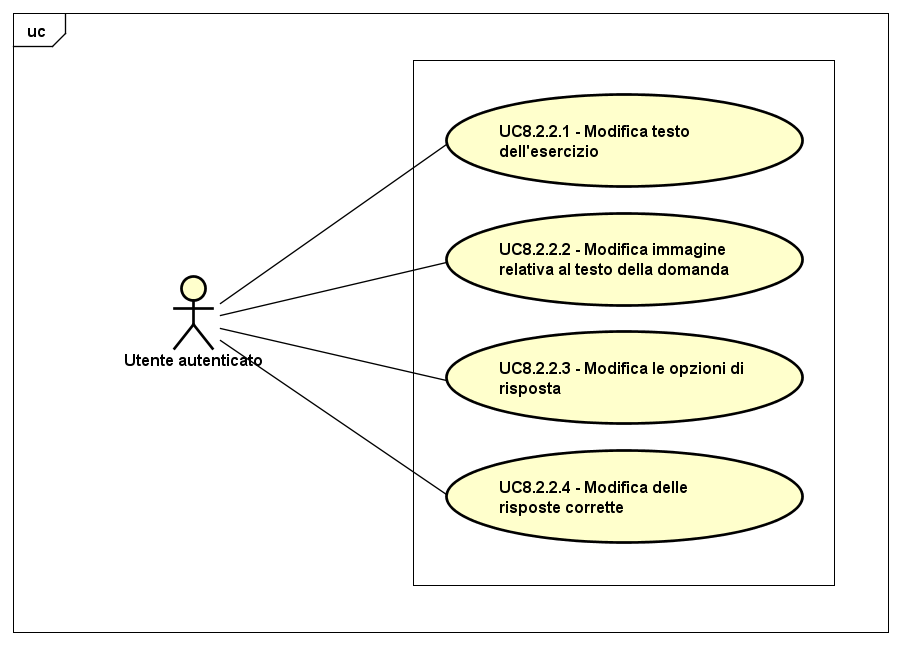
\includegraphics[scale=0.45,keepaspectratio]{UML/UC8_2_2.png}
		\caption{UC8.2.2: Modifica domanda a risposta multipla}
	\end{figure}
	\FloatBarrier
	\begin{itemize}
		\item
			\textbf{Attori}: utente autenticato, utente autenticato pro;
		\item		
			\textbf{Descrizione}: l'attore può utilizzare la procedura guidata per la modifica di una domanda a risposta multipla;
		\item
			\textbf{Precondizione}: il sistema ha ricevuto dall'attore la domanda da modificare;
		\item
			\textbf{Postcondizione}: l'attore ha modificato una domanda a risposta multipla;
		\item
			\textbf{Scenario principale}:
	       		\begin{enumerate}
	       			\item
	       			L'attore può modificare il testo della domanda (UC8.2.2.1);
	       			\item
	       			L'attore può modificare l'immagine relativa al testo della domanda (UC8.2.2.2);
	       			\item
	       			L'attore può modificare le opzioni di risposta (UC8.2.2.3);
					\item
					L'attore può modificare le risposte corrette (UC8.2.2.4).
	 			\end{enumerate}
	\end{itemize}

\subsubsection{Caso d'uso UC8.2.2.1: Modifica testo della domanda}
	\begin{itemize}
		\item
			\textbf{Attori}: utente autenticato, utente autenticato pro;
		\item		
			\textbf{Descrizione}: l'attore può modificare il testo della domanda;
		\item
			\textbf{Precondizione}: il sistema mostra la funzionalità di modifica di una domanda a risposta multipla;
		\item
			\textbf{Postcondizione}: l'attore ha modificato il testo della domanda;
		\item
			\textbf{Scenario principale}: l'attore modifica il testo della domanda. 
	 			
	\end{itemize}
	
\subsubsection{Caso d'uso UC8.2.2.2: Modifica immagine}
	\begin{itemize}
		\item
			\textbf{Attori}: utente autenticato, utente autenticato pro;
		\item		
			\textbf{Descrizione}: l'attore può modificare l'immagine relativa al testo della domanda;
		\item
			\textbf{Precondizione}: il sistema mostra la funzionalità di modifica di una domanda a risposta multipla;
		\item
			\textbf{Postcondizione}: l'attore ha modificato l'immagine relativa al testo della domanda;
		\item
			\textbf{Scenario principale}: l'attore modifica l'immagine relativa al testo della domanda. 	
	\end{itemize}
	
	
\subsubsection{Caso d'uso UC8.2.2.3: Modifica opzioni di risposta}
	\label{UC8.2.2.3}
	\begin{figure}[h]
		\centering
			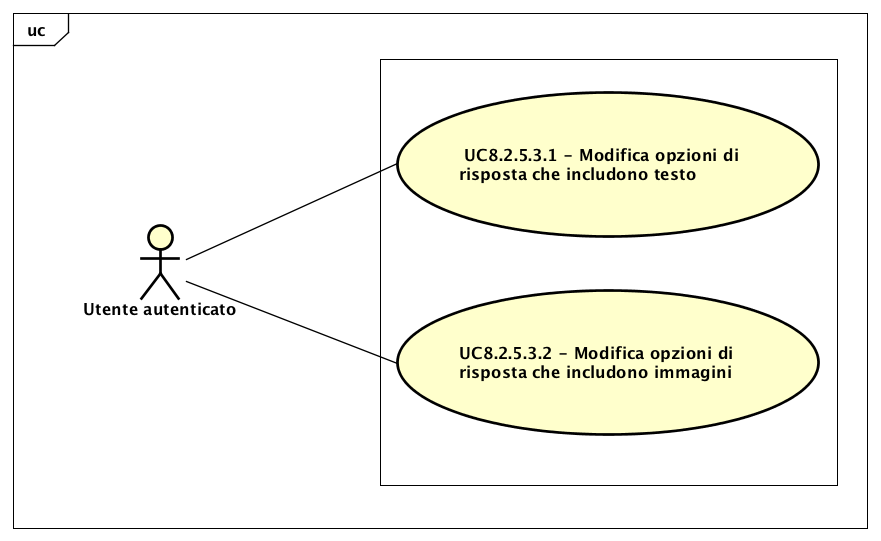
\includegraphics[scale=0.45,keepaspectratio]{UML/UC8_2_2_3.png}
		\caption{UC8.2.2.3: Modifica opzioni di risposta}
	\end{figure}
	\FloatBarrier
	\begin{itemize}
		\item
			\textbf{Attori}: utente autenticato, utente autenticato pro;
		\item		
			\textbf{Descrizione}: l'attore può modificare le opzioni di risposta;
		\item
			\textbf{Precondizione}: il sistema mostra la funzionalità di modifica di una domanda a risposta multipla;
		\item
			\textbf{Postcondizione}: l'attore ha modificato le opzioni di risposta;
		\item
			\textbf{Scenario principale}:
	       		\begin{enumerate}
	       			\item
	       			L'attore può modificare opzioni di risposta che includono testo (UC8.2.2.3.1);
					\item
					L'attore può modificare opzioni di risposta che includono immagini (UC8.2.2.3.2).
	 			\end{enumerate}
	\end{itemize}	
	
\subsubsection{Caso d'uso UC8.2.2.3.1: Modifica opzioni di risposta che includono testo}
	\begin{itemize}
		\item
			\textbf{Attori}: utente autenticato, utente autenticato pro;
		\item		
			\textbf{Descrizione}: l'attore può modificare le opzioni di risposta che includono testo;
		\item
			\textbf{Precondizione}: il sistema mostra la funzionalità di modifica di una domanda a risposta multipla con opzioni di risposta che includono testo; 
		\item
			\textbf{Postcondizione}: l'attore ha modificato le opzioni di risposta che includono testo;
		\item
			\textbf{Scenario principale}: l'attore modifica le opzioni di risposta che includono testo. 			
	\end{itemize}	
	
\subsubsection{Caso d'uso UC8.2.2.3.2: Modifica opzioni di risposta che includono immagini}
	\begin{itemize}
		\item
			\textbf{Attori}: utente autenticato, utente autenticato pro;
		\item		
			\textbf{Descrizione}: l'attore può modificare le opzioni di risposta che includono immagini;
		\item
			\textbf{Precondizione}: il sistema mostra la funzionalità di modifica di una domanda a risposta multipla con opzioni di risposta che includono immagini; 
		\item
			\textbf{Postcondizione}: l'attore ha modificato le opzioni di risposta che includono immagini;
		\item
			\textbf{Scenario principale}: l'attore modifica le opzioni di risposta che includono immagini. 			
	\end{itemize}
	
\subsubsection{Caso d'uso UC8.2.2.4: Modifica risposte corrette}
	\begin{itemize}
		\item
			\textbf{Attori}: utente autenticato, utente autenticato pro;
		\item		
			\textbf{Descrizione}: l'attore può modificare la selezione delle risposte corrette;
		\item
			\textbf{Precondizione}: il sistema mostra la funzionalità di modifica di una domanda a risposta multipla;
		\item
			\textbf{Postcondizione}: l'attore ha modificato la selezione delle risposte corrette;
		\item
			\textbf{Scenario principale}: l'attore modifica la selezione delle risposte corrette. 			
	\end{itemize}

\subsubsection{Caso d'uso UC8.2.3: Modifica esercizio a riempimento di spazi vuoti}
	\label{UC8.2.3}
	\begin{figure}[ht]
		\centering
			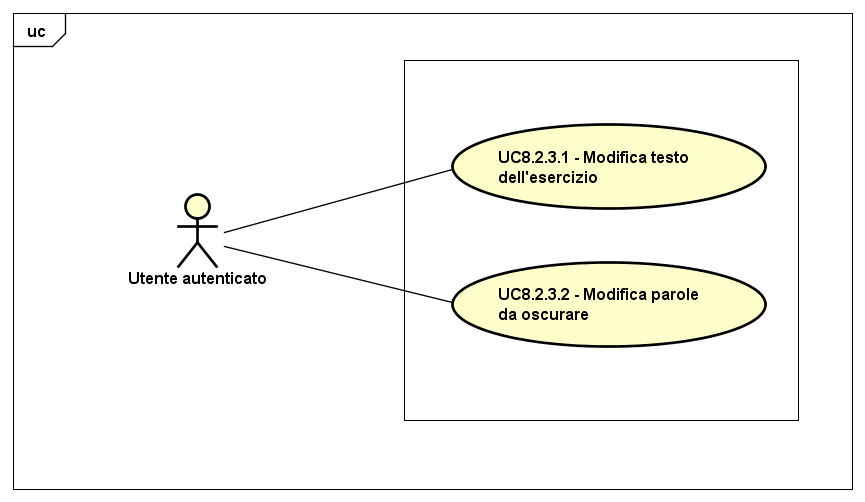
\includegraphics[scale=0.45,keepaspectratio]{UML/UC8_2_3.png}
		\caption{UC8.2.3: Modifica esercizio a riempimento di spazi vuoti}
	\end{figure}
	\FloatBarrier
	\begin{itemize}
		\item
			\textbf{Attori}: utente autenticato, utente autenticato pro;
		\item		
			\textbf{Descrizione}: l'attore può utilizzare la procedura guidata per la modifica di un esercizio a riempimento di spazi vuoti;
		\item
			\textbf{Precondizione}: il sistema ha ricevuto dall'attore la domanda da modificare;
		\item
			\textbf{Postcondizione}: l'attore ha modificato un esercizio a riempimento di spazi vuoti;
		\item
			\textbf{Scenario principale}:
	       		\begin{enumerate}
	       			\item
	       			L'attore può modificare il testo dell'esercizio (UC8.2.3.1);
	       			\item
	       			L'attore può modificare le parole che saranno sostituite con degli spazi vuoti dal sistema (UC8.2.3.2).
	 			\end{enumerate}
	\end{itemize}
	
\subsubsection{Caso d'uso UC8.2.3.1: Modifica testo dell'esercizio}
	\begin{itemize}
		\item
			\textbf{Attori}: utente autenticato, utente autenticato pro;
		\item		
			\textbf{Descrizione}: l'attore può modificare il testo dell'esercizio;
		\item
			\textbf{Precondizione}: il sistema mostra la funzionalità di modifica di un esercizio a riempimento di spazi;
		\item
			\textbf{Postcondizione}: l'attore ha modificato il testo dell'esercizio;
		\item
			\textbf{Scenario principale}: l'attore modifica il testo dell'esercizio.
	\end{itemize}


\subsubsection{Caso d'uso UC8.2.3.2: Modifica parole da oscurare}
	\begin{itemize}
		\item
			\textbf{Attori}: utente autenticato, utente autenticato pro;
		\item		
			\textbf{Descrizione}: l'attore può modificare le parole che saranno sostituite con degli spazi vuoti;
		\item
			\textbf{Precondizione}: il sistema mostra la funzionalità di modifica di un esercizio a riempimento di spazi;
		\item
			\textbf{Postcondizione}: l'attore ha modificato le parole che saranno sostituite con degli spazi vuoti;
		\item
			\textbf{Scenario principale}: l'attore modifica le parole che verranno oscurate dal sistema.
	\end{itemize}

\subsubsection{Caso d'uso UC8.2.4: Modifica domanda di collegamento}
\label{UC8.2.4}
\begin{figure}[ht]
	\centering
	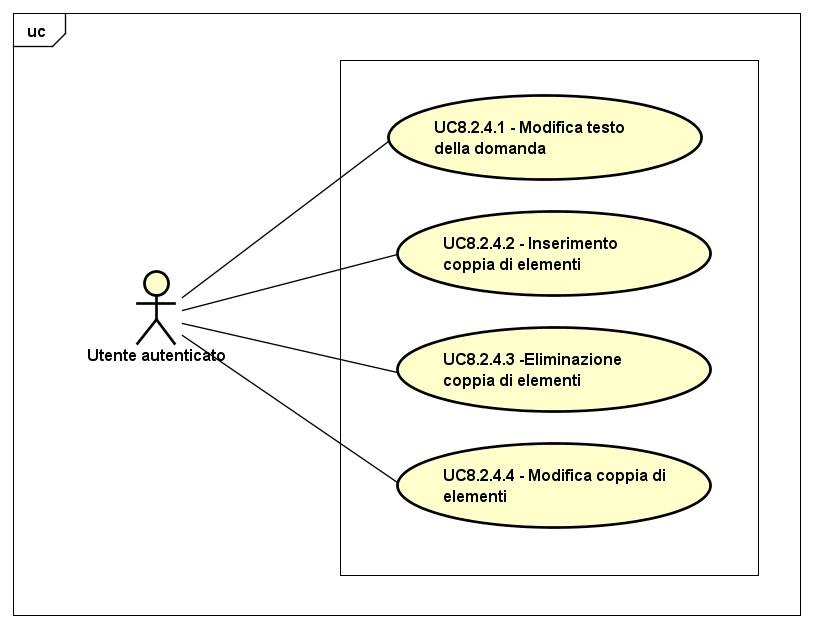
\includegraphics[scale=0.5,keepaspectratio]{UML/UC8_2_4.png}
	\caption{Caso d'uso UC8.2.4: Modifica domanda di collegamento}
\end{figure}
\FloatBarrier
\begin{itemize}
	\item \textbf{Attori}: \uau, \uaupro;
	\item \textbf{Descrizione}: l'attore può utilizzare la procedura guidata per la modifica di una domanda di collegamento; 
	\item \textbf{Precondizione}: il sistema ha ricevuto dall'attore la domanda da modificare; 
	\item \textbf{Postcondizione}: l'attore ha modificato una domanda di collegamento;
	\item \textbf{Scenario principale}: 
	\begin{enumerate}
			\item L'attore può modificare il testo della domanda (UC8.2.4.1);
			\item L'attore può inserire una coppia di elementi (UC8.2.4.2);
			\item L'attore può eliminare una coppia di elementi inserita (UC8.2.4.3);
			\item L'attore può modificare una coppia di elementi inserita (UC8.2.4.4).
		\end{enumerate}
	\item \textbf{Scenari alternativi}: se non ci sono almeno due coppie presenti nella lista delle coppie l'attore deve inserire una nuova coppia di elementi.
\end{itemize}

	\subsubsection{Caso d'uso UC8.2.4.1: Modifica testo della domanda}
	\label{UC8.2.4.1}
	\begin{itemize}
		\item
		\textbf{Attori}: \uau, \uaupro;
		\item		
		\textbf{Descrizione}: l'attore può modificare il testo della domanda;
		\item
		\textbf{Precondizione}: il sistema mostra la funzionalità di modifica di una domanda di collegamento; 
		\item
		\textbf{Postcondizione}: l'attore ha modificato il testo della domanda;
		\item
		\textbf{Scenario principale}: l'attore modifica il testo della domanda.	
	\end{itemize}

	\subsubsection{Caso d'uso UC8.2.4.2: Inserimento coppia di elementi}
	\label{UC8.2.4.2}
	\begin{figure}[h]
		\centering
		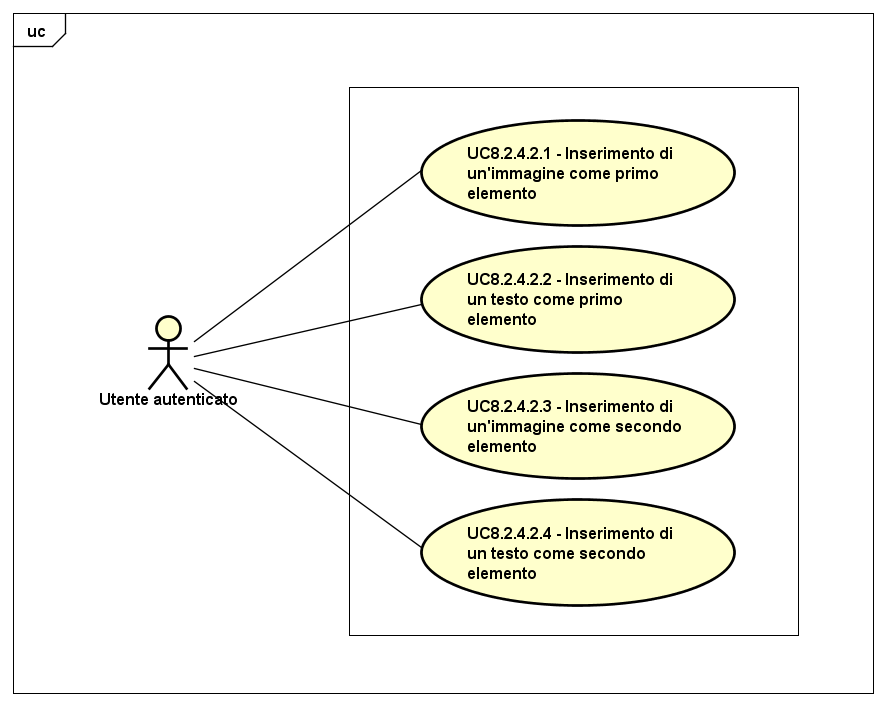
\includegraphics[scale=0.5,keepaspectratio]{UML/UC8_2_4_2.png}
		\caption{Caso d'uso UC8.2.4.2: Inserimento coppia di elementi}
	\end{figure}
	\FloatBarrier
	\begin{itemize}
		\item \textbf{Attori}: \uau, \uaupro;
		\item \textbf{Descrizione}: l'attore può inserire una coppia di elementi, sia immagini che testo o combinazioni di questi, che siano correlati tra loro in modo da indicare la soluzione della domanda; 
		\item \textbf{Precondizione}: il sistema mostra la funzionalità di modifica di una domanda di collegamento; 
		\item \textbf{Postcondizione}: l'attore ha inserito una coppia di elementi nella lista di coppie di elementi; 
		\item \textbf{Scenario principale}: 
		\begin{enumerate}
			\item L'attore inserisce come primo elemento un'immagine (UC8.2.4.2.1);
			\item L'attore inserisce come primo elemento un testo (UC8.2.4.2.2);
			\item L'attore inserisce come secondo elemento un'immagine (UC8.2.4.2.3);
			\item L'attore inserisce come secondo elemento un testo (UC8.2.4.2.4).	
		\end{enumerate}
	\end{itemize}
	
		\subsubsection{Caso d'uso UC8.2.4.2.1: Inserimento di un'immagine come primo elemento}
		\label{UC8.2.4.2.1}
		\begin{itemize}
			\item \textbf{Attori}: \uau, \uaupro;
			\item \textbf{Descrizione}: l'attore può inserire come primo elemento della coppia un'immagine;
			\item \textbf{Precondizione}: il sistema mostra la funzionalità di modifica di una domanda di collegamento; 
			\item \textbf{Postcondizione}: l'attore ha inserito come primo elemento un'immagine;
			\item \textbf{Scenario principale}: l'attore carica un'immagine come primo elemento della coppia.
		\end{itemize}
		
		\subsubsection{Caso d'uso UC8.2.4.2.2: Inserimento di un testo come primo elemento}
		\label{UC8.2.4.2.2}
		\begin{itemize}
			\item \textbf{Attori}: \uau, \uaupro;
			\item \textbf{Descrizione}: l'attore può inserire come primo elemento della coppia un testo;
			\item \textbf{Precondizione}: il sistema mostra la funzionalità di modifica di una domanda di collegamento; 
			\item \textbf{Postcondizione}: l'attore ha inserito come primo elemento un testo;
			\item \textbf{Scenario principale}: l'attore inserisce del testo come primo elemento della coppia.
		\end{itemize}
		
			\subsubsection{Caso d'uso UC8.2.4.2.3: Inserimento di un'immagine come secondo elemento}
		\label{UC8.2.4.2.3}
		\begin{itemize}
			\item \textbf{Attori}: \uau, \uaupro;
			\item \textbf{Descrizione}: l'attore può inserire come secondo elemento della coppia un'immagine;
			\item \textbf{Precondizione}: il sistema mostra la funzionalità di modifica di una domanda di collegamento; 
			\item \textbf{Postcondizione}: l'attore ha inserito come secondo elemento un'immagine;
			\item \textbf{Scenario principale}: l'attore carica un'immagine come secondo elemento della coppia.
		\end{itemize}
		
		\subsubsection{Caso d'uso UC8.2.4.2.4: Inserimento di un testo come secondo elemento}
		\label{UC8.2.4.2.4}
		\begin{itemize}
			\item \textbf{Attori}: \uau, \uaupro;
			\item \textbf{Descrizione}: l'attore può inserire come secondo elemento della coppia un testo;
			\item \textbf{Precondizione}:il sistema mostra la funzionalità di modifica di una domanda di collegamento; 
			\item \textbf{Postcondizione}: l'attore ha inserito come secondo elemento un testo;
			\item \textbf{Scenario principale}: l'attore inserisce del testo come secondo elemento della coppia.
		\end{itemize}
	
	\subsubsection{Caso d'uso UC8.2.4.3: Eliminazione coppia di elementi}
	\label{UC8.2.4.3}
	\begin{figure}[h]
		\centering
		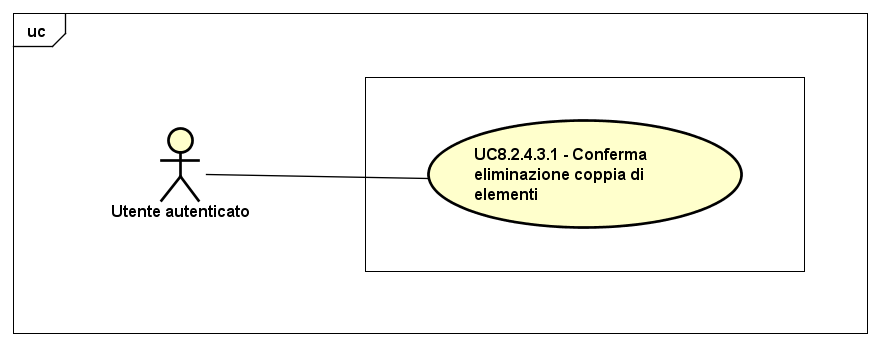
\includegraphics[scale=0.5,keepaspectratio]{UML/UC8_2_4_3.png}
		\caption{Caso d'uso UC8.2.4.3: Eliminazione coppia di elementi}
	\end{figure}
	\FloatBarrier
	\begin{itemize}
		\item \textbf{Attori}: \uau, \uaupro;
		\item \textbf{Descrizione}: l'attore può rimuovere una coppia di elementi dalla lista di coppie di elementi;
		\item \textbf{Precondizione}: il sistema mostra la funzionalità di modifica di una domanda di collegamento; 
		\item \textbf{Postcondizione}: l'attore ha eliminato una coppia di elementi dalla lista delle coppie di elementi;
		\item \textbf{Scenario principale}: l'attore può confermare l'eliminazione di una coppia di elementi (UC8.2.4.3.1);
		\item \textbf{Scenari alternativi}: l'attore annulla l'operazione tornando alla schermata precedente.
	\end{itemize}

		\subsubsection{Caso d'uso UC8.2.4.3.1: Conferma eliminazione coppia di elementi}
		\label{UC8.2.4.3.1}
		\begin{itemize}
			\item \textbf{Attori}: \uau, \uaupro;
			\item \textbf{Descrizione}: l'attore può confermare la rimozione di una coppia di elementi;
			\item \textbf{Precondizione}: il sistema mostra la funzionalità di modifica di una domanda di collegamento; 
			\item \textbf{Postcondizione}: l'attore ha confermato l'eliminazione della coppia di elementi;
			\item \textbf{Scenario principale}: l'attore conferma la rimozione della coppia di elementi.
		\end{itemize}

	\subsubsection{Caso d'uso UC8.2.4.4: Modifica coppia di elementi}
	\label{UC8.2.4.4}
	\begin{figure}[h]
		\centering
		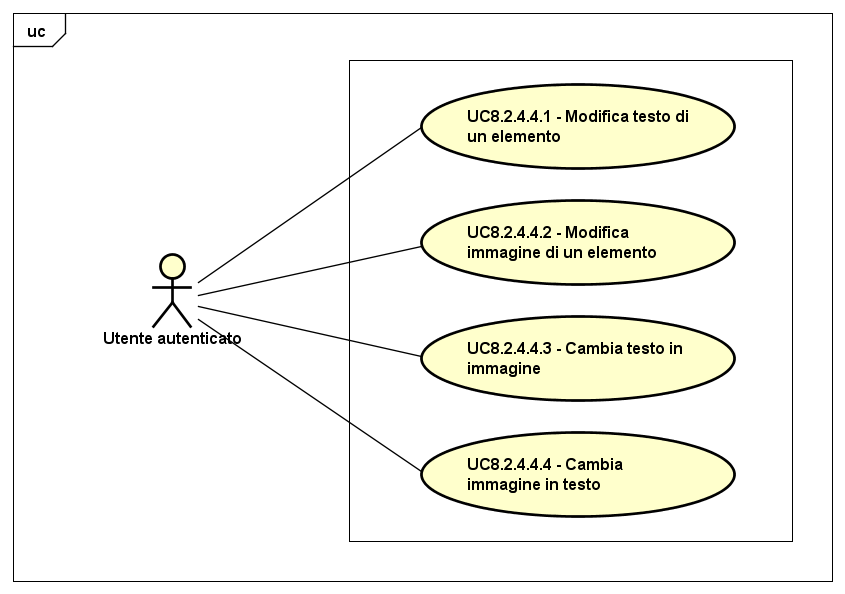
\includegraphics[scale=0.5,keepaspectratio]{UML/UC8_2_4_4.png}
		\caption{Caso d'uso UC8.2.4.4: Modifica coppia di elementi}
	\end{figure}
	\FloatBarrier
	\begin{itemize}
		\item \textbf{Attori}: \uau, \uaupro;
		\item \textbf{Descrizione}: l'attore può modificare una coppia di elementi presente nella lista di coppie di elementi;
		\item \textbf{Precondizione}: il sistema mostra la funzionalità di modifica di una domanda di collegamento; 
		\item \textbf{Postcondizione}: l'attore ha modificato una coppia di elementi presente nella lista di coppie di elementi; 
		\item \textbf{Scenario principale}: 
		\begin{enumerate}
			\item L'attore può modificare un elemento cambiandone il testo (UC8.2.4.4.1);
			\item L'attore può modificare un elemento cambiandone l'immagine (UC8.2.4.4.2);
			\item L'attore può modificare un elemento facendolo passare da testo ad immagine (UC8.2.4.4.3);
			\item L'attore può modificare un elemento facendolo passare da immagine a testo (UC8.2.4.4.4).	
		\end{enumerate}
	\end{itemize}
	
		\subsubsection{Caso d'uso UC8.2.4.4.1: Modifica testo di un elemento}
		\label{UC8.2.4.4.1}
		\begin{itemize}
			\item \textbf{Attori}: \uau, \uaupro;
			\item \textbf{Descrizione}: l'attore può modificare il testo di un elemento;
			\item \textbf{Precondizione}: il sistema mostra la funzionalità di modifica di una domanda di collegamento; 
			\item \textbf{Postcondizione}: l'attore ha modificato il testo di un elemento;
			\item \textbf{Scenario principale}: l'attore modifica il testo di un elemento.  
		\end{itemize}
		
		\subsubsection{Caso d'uso UC8.2.4.4.2: Modifica immagine di un elemento}
		\label{UC8.2.4.4.2}
		\begin{itemize}
			\item \textbf{Attori}: \uau, \uaupro;
			\item \textbf{Descrizione}: l'attore può caricare un'altra immagine per un elemento;
			\item \textbf{Precondizione}: il sistema mostra la funzionalità di modifica di una domanda di collegamento; 
			\item \textbf{Postcondizione}: l'attore ha inserito un'altra immagine per un elemento;
			\item \textbf{Scenario principale}: l'attore carica un'altra immagine per un elemento.
		\end{itemize}
		
		\subsubsection{Caso d'uso UC8.2.4.4.3: Cambia testo in immagine}
		\label{UC8.2.4.4.3}
		\begin{itemize}
			\item \textbf{Attori}: \uau, \uaupro;
			\item \textbf{Descrizione}: l'attore può modificare un elemento facendolo diventare un'immagine al posto di un testo;
			\item \textbf{Precondizione}: il sistema mostra la funzionalità di modifica di una domanda di collegamento; 
			\item \textbf{Postcondizione}: l'attore ha fatto diventare un'immagine un elemento che prima era un testo;
			\item \textbf{Scenario principale}: l'attore inserisce un'immagine come modifica dell'elemento.  
		\end{itemize}
		
		\subsubsection{Caso d'uso UC8.2.4.4.4: Cambia immagine in testo}
		\label{UC8.2.4.4.4}
		\begin{itemize}
			\item \textbf{Attori}: \uau, \uaupro;
			\item \textbf{Descrizione}: l'attore può modificare un elemento facendolo diventare un testo al posto di un'immagine;
			\item \textbf{Precondizione}: il sistema mostra la funzionalità di modifica di una domanda di collegamento; 
			\item \textbf{Postcondizione}: l'attore ha fatto diventare un testo un elemento che prima era un'immagine;
			\item \textbf{Scenario principale}: l'attore inserisce del testo come modifica dell'elemento.  
		\end{itemize}
\subsubsection{Caso d'uso UC8.2.5: Modifica domanda a ordinamento di immagini}
\label{UC8.2.5}
	\begin{figure}[h]
		\centering
			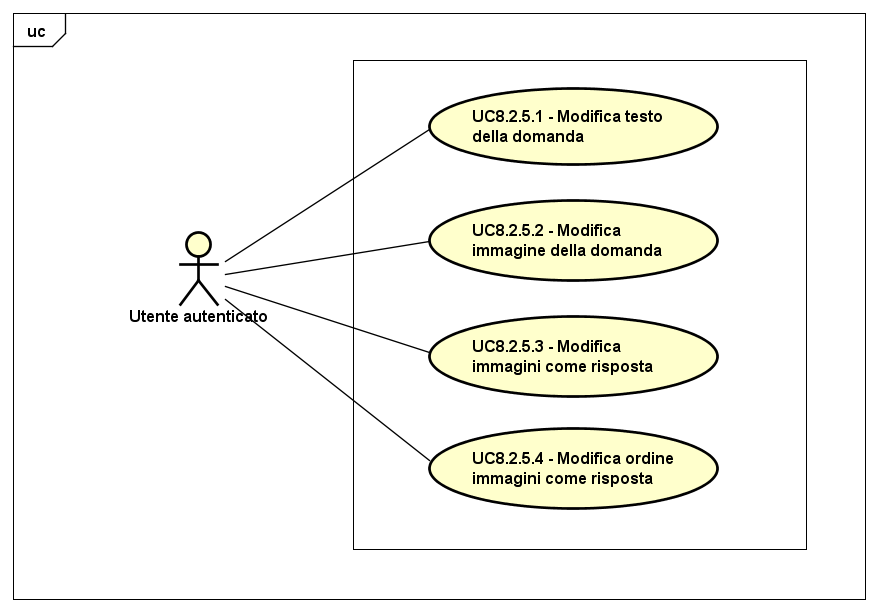
\includegraphics[scale=0.45,keepaspectratio]{UML/UC8_2_5.png}
		\caption{UC8.2.5: Modifica domanda a ordinamento di immagini}
	\end{figure}
\begin{itemize}
	\item\textbf{Attori}: utente autenticato, utente autenticato pro;
	\item\textbf{Descrizione}: l'attore può utilizzare la procedura guidata per la modifica di una domanda a ordinamento di immagini;
	\item\textbf{Precondizione}: il sistema ha ricevuto dall'attore la domanda da modificare; 
	\item \textbf{Postcondizione}: l'attore ha modificato una domanda a ordinamento di immagini;
	\item\textbf{Scenario principale}: 
	\begin{itemize}
		\item L'attore può modificare il testo della domanda (UC8.2.5.1);
		\item L'attore può modifica l'immagine relativa al testo della domanda (UC8.2.5.2);
		\item L'attore può modificare le immagini della sequenza che costituirà la risposta (UC8.2.5.3);
		\item L'attore può modifica l'ordine corretto delle immagini che costituiscono la risposta (UC8.2.5.4).
	\end{itemize}
\end{itemize}

\subsubsection{Caso d'uso UC8.2.5.1: Modifica testo della domanda}
\begin{itemize}
	\item\textbf{Attori}: utente autenticato, utente autenticato pro;
	\item \textbf{Descrizione}: l'attore può modificare il testo della domanda;
		\item
			\textbf{Precondizione}: il sistema mostra la funzionalità di modifica di una domanda a ordinamento di immagini; 
		\item
			\textbf{Postcondizione}: l'attore ha modificato il testo della domanda;
		\item
			\textbf{Scenario principale}: l'attore modifica il testo della domanda.	
	\end{itemize}

\subsubsection{Caso d'uso UC8.2.5.2: Modifica immagine della domanda}
\begin{itemize}
	\item\textbf{Attori}: utente autenticato, utente autenticato pro;
	\item \textbf{Descrizione}: l'attore può modificare l'immagine relativa al testo della domanda;
		\item
			\textbf{Precondizione}: il sistema mostra la funzionalità di modifica di una domanda di ordinamento immagini; 
		\item
			\textbf{Postcondizione}: l'attore ha modificato l'immagine relativa al testo della domanda;
		\item
			\textbf{Scenario principale}: l'attore modifica l'immagine relativa al testo della domanda. 	
	\end{itemize}

\subsubsection{Caso d'uso UC8.2.5.3: Modifica immagini come risposta}
\begin{itemize}
	\item\textbf{Attori}: utente autenticato, utente autenticato pro;
	\item\textbf{Descrizione}: l'attore può modificare le immagini che costituiscono la risposta alla domanda sostituendole con delle altre;
	\item\textbf{Precondizione}: il sistema mostra la funzionalità di modifica di una domanda di ordinamento immagini;  
	\item \textbf{Postcondizione}: l'attore ha inserito nuove immagini come risposta alla domanda;
	\item\textbf{Scenario principale}: l'attore sostituisce le immagini presenti come risposta alla domanda con delle altre.
\end{itemize}

\subsubsection{Caso d'uso UC8.2.5.4: Modifica ordine immagini come risposta}
\begin{itemize}
	\item\textbf{Attori}: utente autenticato, utente autenticato pro;
	\item\textbf{Descrizione}: l'attore può modificare l'ordine corretto delle immagini che rappresenta la soluzione della domanda;
	\item\textbf{Precondizione}: il sistema mostra la funzionalità di modifica di una domanda di ordinamento immagini; 
	\item \textbf{Postcondizione}: l'attore ha modificato l'ordine delle immagini che costituiscono la risposta alla domanda;
	\item\textbf{Scenario principale}: l'attore modifica l'ordine delle immagini che costituiscono la risposta alla domanda.
\end{itemize}

\subsubsection{Caso d’uso UC8.2.6: Modifica domanda a ordinamento di stringhe}
	\label{UC8.2.6}
	\begin{figure}[h]
		\centering
		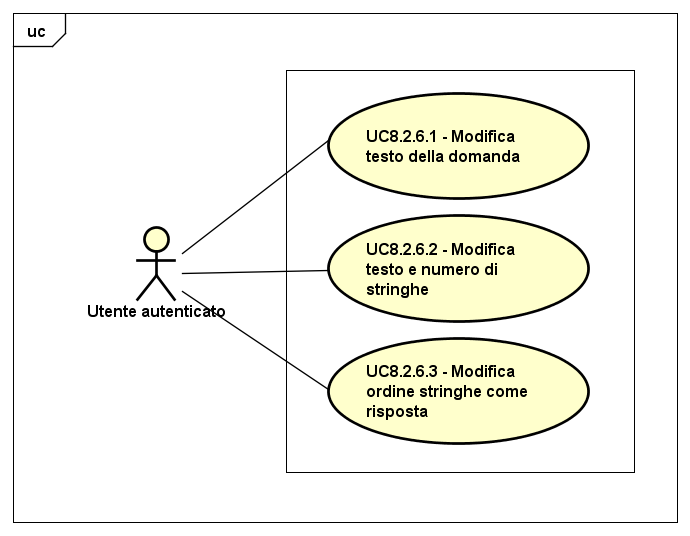
\includegraphics[scale=0.45,keepaspectratio]{UML/UC8_2_6.png}
		\caption{UC8.2.6: Modifica domanda a ordinamento di stringhe}
	\end{figure}
	\FloatBarrier
\begin{itemize}
	\item\textbf{Attori}: utente autenticato, utente autenticato pro;
	\item\textbf{Descrizione}: l'attore può utilizzare la procedura guidata per la modifica di una domanda a ordinamento di stringhe;
	\item\textbf{Precondizione}: il sistema ha ricevuto dall'attore la domanda da modificare; 
	\item \textbf{Postcondizione}: l'attore ha modificato una domanda a ordinamento di stringhe;
	\item\textbf{Scenario principale}:
		\begin{itemize}
			\item L'attore può modificare il testo della domanda (UC8.2.6.1);
			\item L'attore può modificare il testo e il numero delle stringhe che compongono la sequenza della domanda (UC8.2.6.2);
			\item L'attore può modificare l'ordine corretto delle stringhe che costituiscono la risposta (UC8.2.6.3).
		\end{itemize}
\end{itemize}

\subsubsection{Caso d'uso UC8.2.6.1: Modifica testo della domanda}
\begin{itemize}
	\item \textbf{Attori}: utente autenticato, utente autenticato pro;
	\item \textbf{Descrizione}: l'attore può modificare il testo della domanda;
	\item \textbf{Precondizione}:  il sistema mostra la funzionalità di modifica di una domanda a ordinamento di stringhe; 
	\item \textbf{Postcondizione}: l'attore ha modificato il testo della domanda;
	\item \textbf{Scenario principale}: l'attore modifica il testo della domanda.
\end{itemize}

\subsubsection{Caso d'uso UC8.2.6.2: Modifica testo e numero di stringhe}
\begin{itemize}
	\item \textbf{Attori}: utente autenticato, utente autenticato pro;
	\item \textbf{Descrizione}: l'attore può modificare il testo e il numero di stringhe che costituiscono la risposta alla domanda;
	\item \textbf{Precondizione}:  il sistema mostra la funzionalità di modifica di una domanda a ordinamento di stringhe;
	\item \textbf{Postcondizione}: l'attore ha modificato il testo e il numero delle stringhe che costituiscono la risposta alla domanda;
	\item \textbf{Scenario principale}: l'attore modifica il testo e il numero delle stringhe che costituiscono la risposta alla domanda.
\end{itemize}

\subsubsection{Caso d'uso UC8.2.6.3: Modifica ordine stringhe come risposta}
\begin{itemize}
	\item \textbf{Attori}: utente autenticato, utente autenticato pro;
	\item \textbf{Descrizione}: l'attore può modificare l'ordine corretto delle stringhe che rappresenta la soluzione della domanda;
	\item \textbf{Precondizione}:  il sistema mostra la funzionalità di modifica di una domanda a ordinamento di stringhe; 
	\item \textbf{Postcondizione}: l'attore ha modificato l'ordine delle stringhe che costituiscono la risposta alla domanda;
	\item \textbf{Scenario principale}: l'attore modifica l'ordine delle stringhe che costituiscono la risposta alla domanda.
\end{itemize}

\subsubsection{Caso d'uso UC8.2.7: Modifica domanda con area cliccabile nell'immagine}
\label{UC8.2.7}
\begin{figure}[ht]
	\centering
	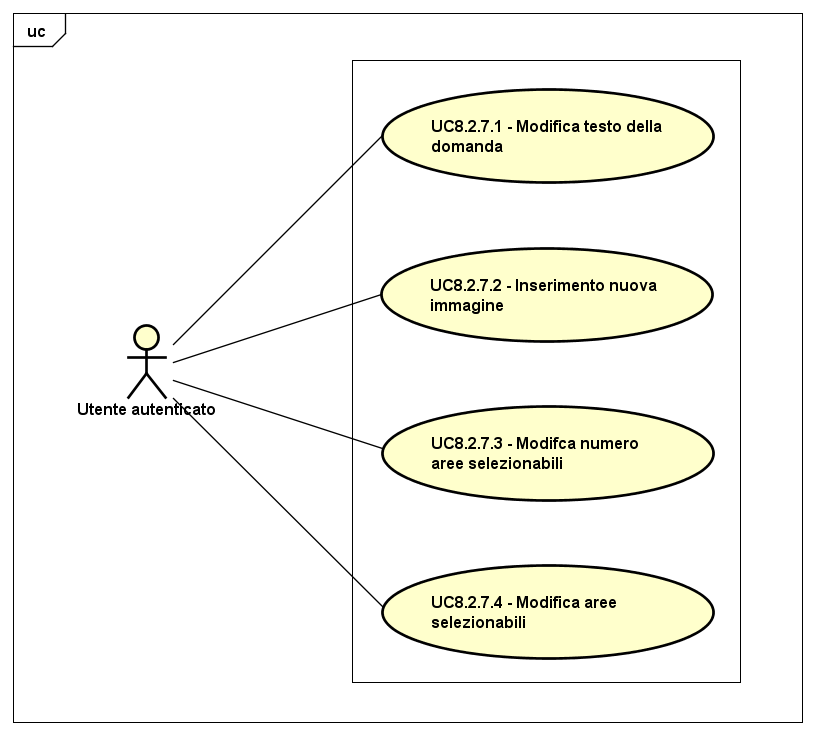
\includegraphics[scale=0.5,keepaspectratio]{UML/UC8_2_7.png}
	\caption{UC8.2.7: Modifica domanda con area cliccabile nell'immagine}
\end{figure}
\FloatBarrier
\begin{itemize}
	\item \textbf{Attori}: utente autenticato, utente autenticato pro;
	\item \textbf{Descrizione}: l'attore può utilizzare la procedura guidata per la modifica di una domanda la cui risposta è selezionabile all'interno di aree cliccabili in un'immagine;
	\item \textbf{Precondizione}:  il sistema ha ricevuto dall'attore la domanda da modificare; 
	\item \textbf{Postcondizione}: l'attore ha modificato una domanda con area cliccabile nell'immagine;
	\item \textbf{Scenario principale}:
		\begin{enumerate}
	       	\item L'attore può modificare il testo della domanda (UC8.2.7.1);
	        \item L'attore può modificare l'immagine relativa al testo della domanda (UC8.2.7.2);
			\item L'attore può scegliere un nuovo numero di aree che saranno selezionabili all'interno dell'immagine (UC8.2.7.3);
			\item L'attore può scegliere nuove aree selezionabili all'interno dell'immagine (UC8.2.7.4);
	 	\end{enumerate}
\end{itemize}

\subsubsection{Caso d'uso UC8.2.7.1: Modifica testo della domanda}
\begin{itemize}
	\item \textbf{Attori}: utente autenticato, utente autenticato pro;
	\item \textbf{Descrizione}: l'attore può modificare il testo della domanda;
	\item \textbf{Precondizione}: il sistema mostra la funzionalità di modifica di una domanda con area cliccabile nell'immagine; 
	\item \textbf{Postcondizione}: l'attore ha modificato il testo della domanda;
	\item \textbf{Scenario principale}: l'attore modifica il testo della domanda. 
\end{itemize}

\subsubsection{Caso d'uso UC8.2.7.2: Inserimento nuova immagine}
\begin{itemize}
	\item \textbf{Attori}: utente autenticato, utente autenticato pro;
	\item \textbf{Descrizione}: l'attore può inserire una nuova immagine relativa al testo della domanda che sostituisce quella già presente;
	\item \textbf{Precondizione}: il sistema mostra la funzionalità di modifica di una domanda con area cliccabile nell'immagine; 
	
	\item \textbf{Postcondizione}: l'attore ha inserito una nuova immagine;
	\item \textbf{Scenario principale}: l'attore inserisce una nuova immagine al posto di quella che era presente. 	
\end{itemize}

\subsubsection{Caso d'uso UC8.2.7.3: Modifica numero aree selezionabili}
\begin{itemize}
	\item \textbf{Attori}: utente autenticato, utente autenticato pro;
	\item \textbf{Descrizione}: l'attore può scegliere un nuovo numero di aree selezionabili all'interno dell'immagine;
	\item \textbf{Precondizione}: il sistema mostra la funzionalità di modifica di una domanda con area cliccabile nell'immagine; 
	
	\item \textbf{Postcondizione}: l'attore ha scelto il nuovo numero di aree selezionabili all'interno dell'immagine;
	\item \textbf{Scenario principale}: l'attore sceglie il nuovo numero di aree selezionabili all'interno dell'immagine. 	
\end{itemize}

\subsubsection{Caso d'uso UC8.2.7.4: Modifica aree selezionabili}
\begin{itemize}
	\item \textbf{Attori}: utente autenticato, utente autenticato pro;
	\item \textbf{Descrizione}: l'attore può scegliere dove inserire le nuove aree selezionabili o riposizionare quelle già presenti all'interno dell'immagine;
	\item \textbf{Precondizione}: il sistema mostra la funzionalità di modifica di una domanda con area cliccabile nell'immagine; 
	
	\item \textbf{Postcondizione}: l'attore ha scelto dove inserire le nuove aree selezionabili o dove riposizionare quelle già presenti all'interno dell'immagine;
	\item \textbf{Scenario principale}: l'attore sceglie dove inserire le nuove aree selezionabili o riposiziona quelle già presenti all'interno dell'immagine. 	
\end{itemize}


	\subsubsection{Caso d'uso UC8.2.8: Conferma modifica}
	\begin{itemize}
		\item
		\textbf{Attori}: utente autenticato, utente autenticato pro;
		\item
		\textbf{Descrizione}: l'attore può confermare la modifica della domanda;
		\item		
		\textbf{Precondizione}: l'attore ha finito di modificare una domanda tramite un \textit{wizard\ped{G}};
		\item
		\textbf{Postcondizione}: l'attore ha modificato una domanda;
		\item
		\textbf{Scenario principale}: l'attore conferma la modifica della domanda;		
		\item
		\textbf{Scenari alternativi}: l'attore annulla la modifica della domanda.
	\end{itemize}		
	\subsubsection{Caso d'uso UC8.2.9: Visualizzazione errore modifica}
	\begin{itemize}
		\item
		\textbf{Attori}: utente autenticato, utente autenticato pro;
		\item
		\textbf{Descrizione}: l'attore può visualizzare un messaggio d'errore nel caso si fossero verificati uno o più scenari alternativi durante la modifica della domanda;
		\item		
		\textbf{Precondizione}: il sistema ha ricevuto dei dati errati per la modifica della domanda;
		\item
		\textbf{Postcondizione}: il sistema avvisa l'attore dell'errore verificatosi tramite un opportuno messaggio;
		\item
		\textbf{Scenario principale}: l'attore visualizza un messaggio d'errore.	
	\end{itemize}	

	\subsubsection{Caso d'uso UC8.3: Creazione nuova domanda tramite editor di testo QML}
	\label{UC8.3}
	\begin{figure}[h]
		\centering
		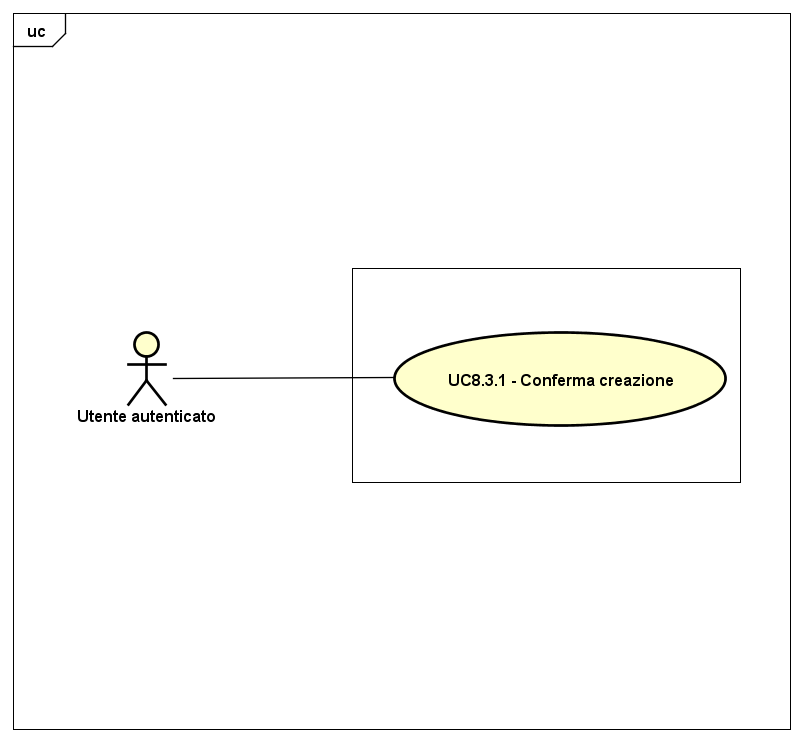
\includegraphics[scale=0.45,keepaspectratio]{UML/UC8_3.png}
		\caption{UC8.3: Creazione nuova domanda tramite editor di testo QML}
	\end{figure}
	\FloatBarrier
	\begin{itemize}
		\item
		\textbf{Attori}: utente autenticato, utente autenticato pro;
		\item		
		\textbf{Descrizione}: l'attore può creare una nuova domanda tramite un editor di testo \textit{QML\ped{G}};
		\item
		\textbf{Precondizione}: il sistema presenta la funzionalità di creazione della domanda;
		\item
		\textbf{Postcondizione}: l'attore crea una domanda;		
		\item
		\textbf{Scenario principale}: l'attore può confermare la creazione della domanda (UC8.3.1).
		\item
		\textbf{Estensioni}: l'attore visualizza un messaggio d'errore relativo alla creazione della domanda (UC8.1.12).
	\end{itemize}	
	
		\subsubsection{Caso d'uso UC8.3.1: Conferma creazione}
		\begin{itemize}
			\item
			\textbf{Attori}: utente autenticato, utente autenticato pro;
			\item
			\textbf{Descrizione}: l'attore può confermare la creazione della domanda effettuata con un editor di testo QML;
			\item		
			\textbf{Precondizione}: l'attore ha finito di modificare una domanda tramite editor di testo \textit{QML\ped{G}};
			\item
			\textbf{Postcondizione}: l'attore ha creato una domanda;
			\item
			\textbf{Scenario principale}: l'attore conferma la creazione della domanda;		
			\item
			\textbf{Scenari alternativi}: l'attore annulla la creazione della domanda.	
		\end{itemize}
	
	\subsubsection{Caso d'uso UC8.4: Modifica domanda esistente tramite editor di testo QML}
	\label{UC8.4}
	\begin{figure}[h]
		\centering
		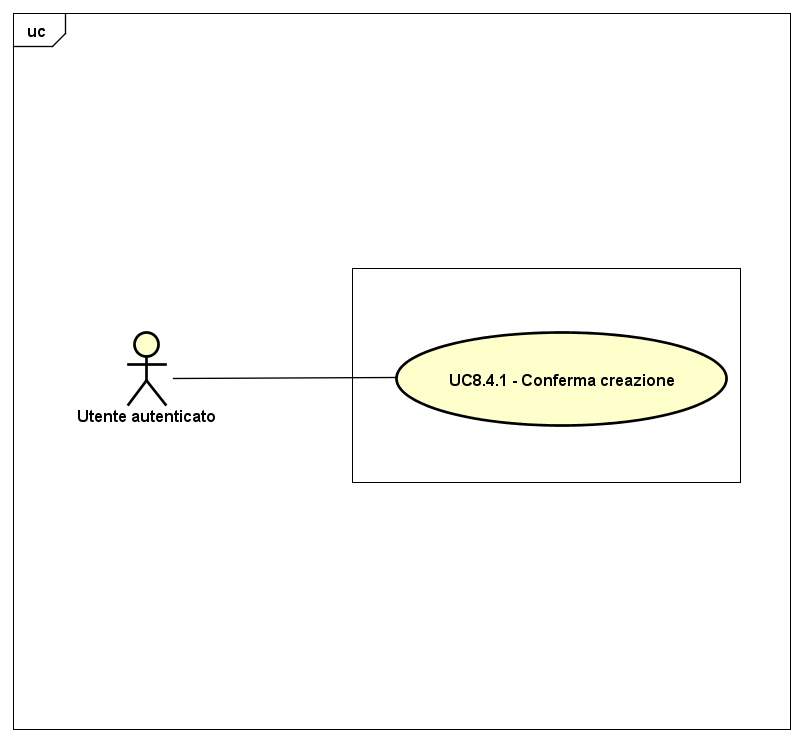
\includegraphics[scale=0.41,keepaspectratio]{UML/UC8_4.png}
		\caption{UC8.4: Modifica domanda esistente tramite editor di testo QML
			}
	\end{figure}
	\FloatBarrier
	\begin{itemize}
		\item
		\textbf{Attori}: utente autenticato, utente autenticato pro;
		\item		
		\textbf{Descrizione}: l'attore può modificare, tramite procedura guidata, una domanda che aveva creato precedentemente;
		\item
		\textbf{Precondizione}: il sistema visualizza la schermata di modifica di una domanda;
		\item
		\textbf{Postcondizione}: l'attore modifica una domanda;
		\item
		\textbf{Scenario principale}: l'attore può confermare le modifiche apportate (UC8.4.1).
	\end{itemize}
		
		\subsubsection{Caso d'uso UC8.4.1: Conferma modifica}
		\begin{itemize}
			\item
			\textbf{Attori}: utente autenticato, utente autenticato pro;
			\item
			\textbf{Descrizione}: l'attore può confermare la modifica della domanda effettuata con un editor di testo QML;
			\item		
			\textbf{Precondizione}: l'attore ha finito di modificare una domanda tramite editor di testo \textit{QML\ped{G}};
			\item
			\textbf{Postcondizione}: l'attore ha modificato una domanda;
			\item
			\textbf{Scenario principale}: l'attore conferma la modifica della domanda;		
			\item
			\textbf{Scenari alternativi}: l'attore annulla la modifica della domanda.
		\end{itemize}
		
	\subsubsection{Caso d'uso UC8.5: Selezione argomento}
	\begin{itemize}
		\item
		\textbf{Attori}: utente autenticato, utente autenticato pro;
		\item
		\textbf{Descrizione}: l'attore può indicare un argomento tra quelli presenti;
		\item		
		\textbf{Precondizione}: il sistema presenta la funzionalità di selezionare un argomento;
		\item
		\textbf{Postcondizione}: l'attore ha selezionato un argomento;
		\item
		\textbf{Scenario principale}: l'attore seleziona l'argomento da assegnare alla nuova domanda.		
	\end{itemize}
	
	\subsubsection{Caso d'uso UC8.6: Inserimento parole chiave}
	\begin{itemize}
		\item
		\textbf{Attori}: utente autenticato, utente autenticato pro;
		\item
		\textbf{Descrizione}: l'attore può inserire le parole chiave relative alla nuova domanda per specificare più dettagliatamente l'argomento della domanda;
		\item		
		\textbf{Precondizione}: il sistema presenta lo spazio destinato all'inserimento di una parola chiave;
		\item
		\textbf{Postcondizione}: l'attore ha selezionato delle parole chiave;
		\item
		\textbf{Scenario principale}: l'attore inserisce delle parole chiave relative alla nuova domanda.	
	\end{itemize}
	
	\subsubsection{Caso d'uso UC8.7: Selezione domande da modificare}
	\begin{itemize}
		\item \textbf{Attori}: utente autenticato, utente autenticato pro;
		\item \textbf{Descrizione}: l'attore può selezionare la domanda da modificare;
		\item \textbf{Precondizione}: il sistema mostra la schermata di selezione della domanda da modificare;
		\item \textbf{Postcondizione}: il sistema ha ricevuto dall'attore la domanda da modificare; 
		\item \textbf{Scenario principale}: l'attore seleziona la domanda da modificare.
		
	\end{itemize}
